\section{Progrès réalisé}

\subsection{I.A. - Intelligence Artificielle}
\setlength{\parindent}{5ex}
Pour implémenter une intelligence artificielle, nous avons testé divers algorithmes de ''pathfinding'' dans un grand nombre de scènes comprenant des obstacles afin de pouvoir implémenter dans notre jeu une entité antagoniste qui suivra le joueur.

\begin{figure}[H]
\centering
\begin{minipage}{.5\textwidth}
  \centering
  \centerline{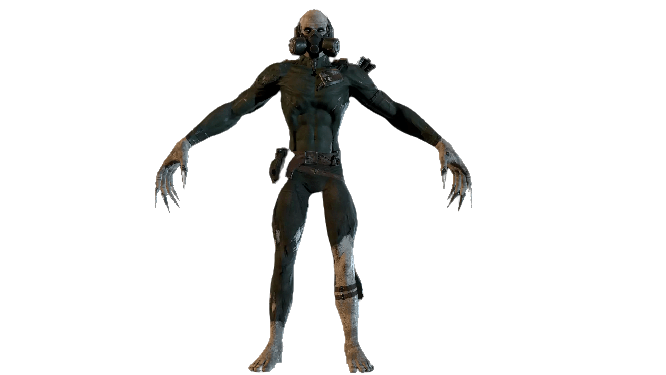
\includegraphics[width=1\linewidth]{img/assets/sterven.png}}
  \captionof{figure}{\emph{Entité}}
  \label{fig:méchant}
\end{minipage}%
\end{figure}

Notre entité utilise le pathfinding pour déterminer, dès lors que le joueur rentrer dans son champ d'action, un chemin à suivre pour atteindre le joueur et l'attaquer.

\begin{figure}[H]
\centering
\begin{minipage}{.5\textwidth}
  \centering
  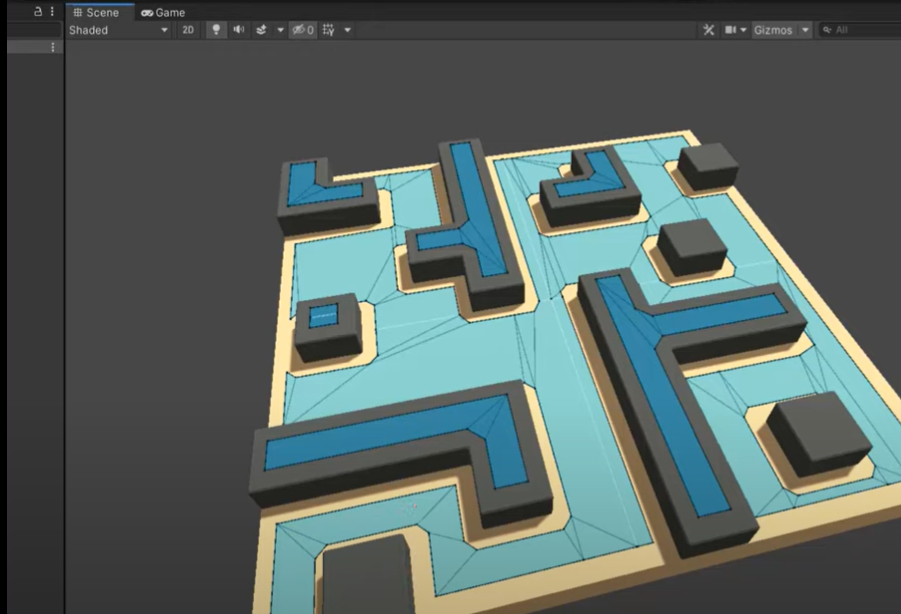
\includegraphics[width=.7\linewidth]{img/navmesh.PNG}
  \captionof{figure}{\emph{NavMesh : Tous les endroits possibles au déplacement de l'entité}}
  \label{fig:navmesh}
\end{minipage}%
\begin{minipage}{.5\textwidth}
  \centering
  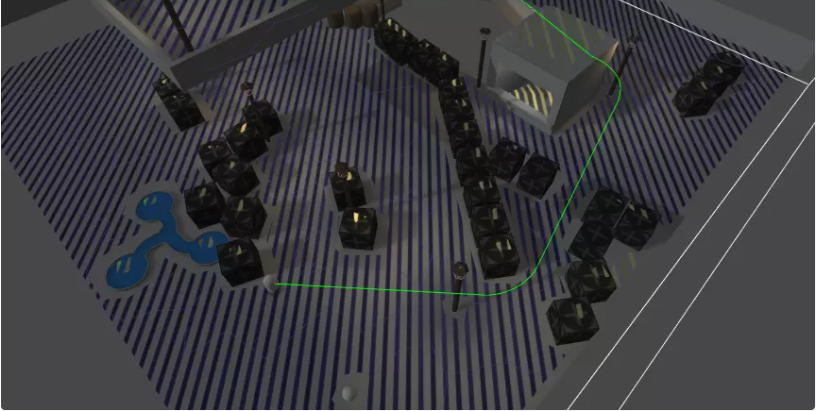
\includegraphics[width=.7\linewidth]{img/path.png}
  \captionof{figure}{\emph{Pathfinding}}
  \label{fig:pathfinding}
\end{minipage}
\end{figure}

Cet intelligence artificielle est utilisée dans le chapitre 3 du jeu.

\vfill
\noindent\makebox[\linewidth]{\rule{.8\paperwidth}{.6pt}}\\[0.2cm]
EPITA Toulouse - Projet S2 - 2022 \hfill Nyctalopia - gameHUB
\noindent\makebox[\linewidth]{\rule{.8\paperwidth}{.6pt}}

\newpage

\subsection{Audio et Effets Sonores}
\setlength{\parindent}{5ex}
La cinématique principale et le menu d’accueil du jeu comptent avec ses propres musiques, libres de droits et utilisables pour usage commercial, qui représentent bien l’aspect mystérieux et effrayant de notre jeu d’horreur.

Le menu d'accueil et l'interface d'utilisateur ont aussi leurs propres effets sonores.

Dans le jeu, le joueur entendra pendant tout le jeu de la musique d'ambiance en arrière-plan correspondant à l'environnement dans lequel il se trouve. Cette musique d'ambiance provenant de \emph{YouTube} est reproduite en boucle et est libre de droits. Des effets sonores circonstanciels peuvent aussi être rencontrés dès que le joueur traverse une zone ou dès lorsqu'il active un des déclencheurs de sons qui sont là pour effrayer le joueur.

Par ailleurs, dès que le joueur rapprochera une borne de sauvegarde, il le saura à cause de la musique qui provient de celle-ci. Pour rendre hommage au jeu vidéo \emph{Fallout 3}, cette chanson est \emph{I Don't Want to Set the World on Fire} de \emph{The Ink Spots}. Il s'agit bien d'une musique libre de droits.

\begin{figure}[H]
\centering
\begin{minipage}{.5\textwidth}
  \centering
  \centerline{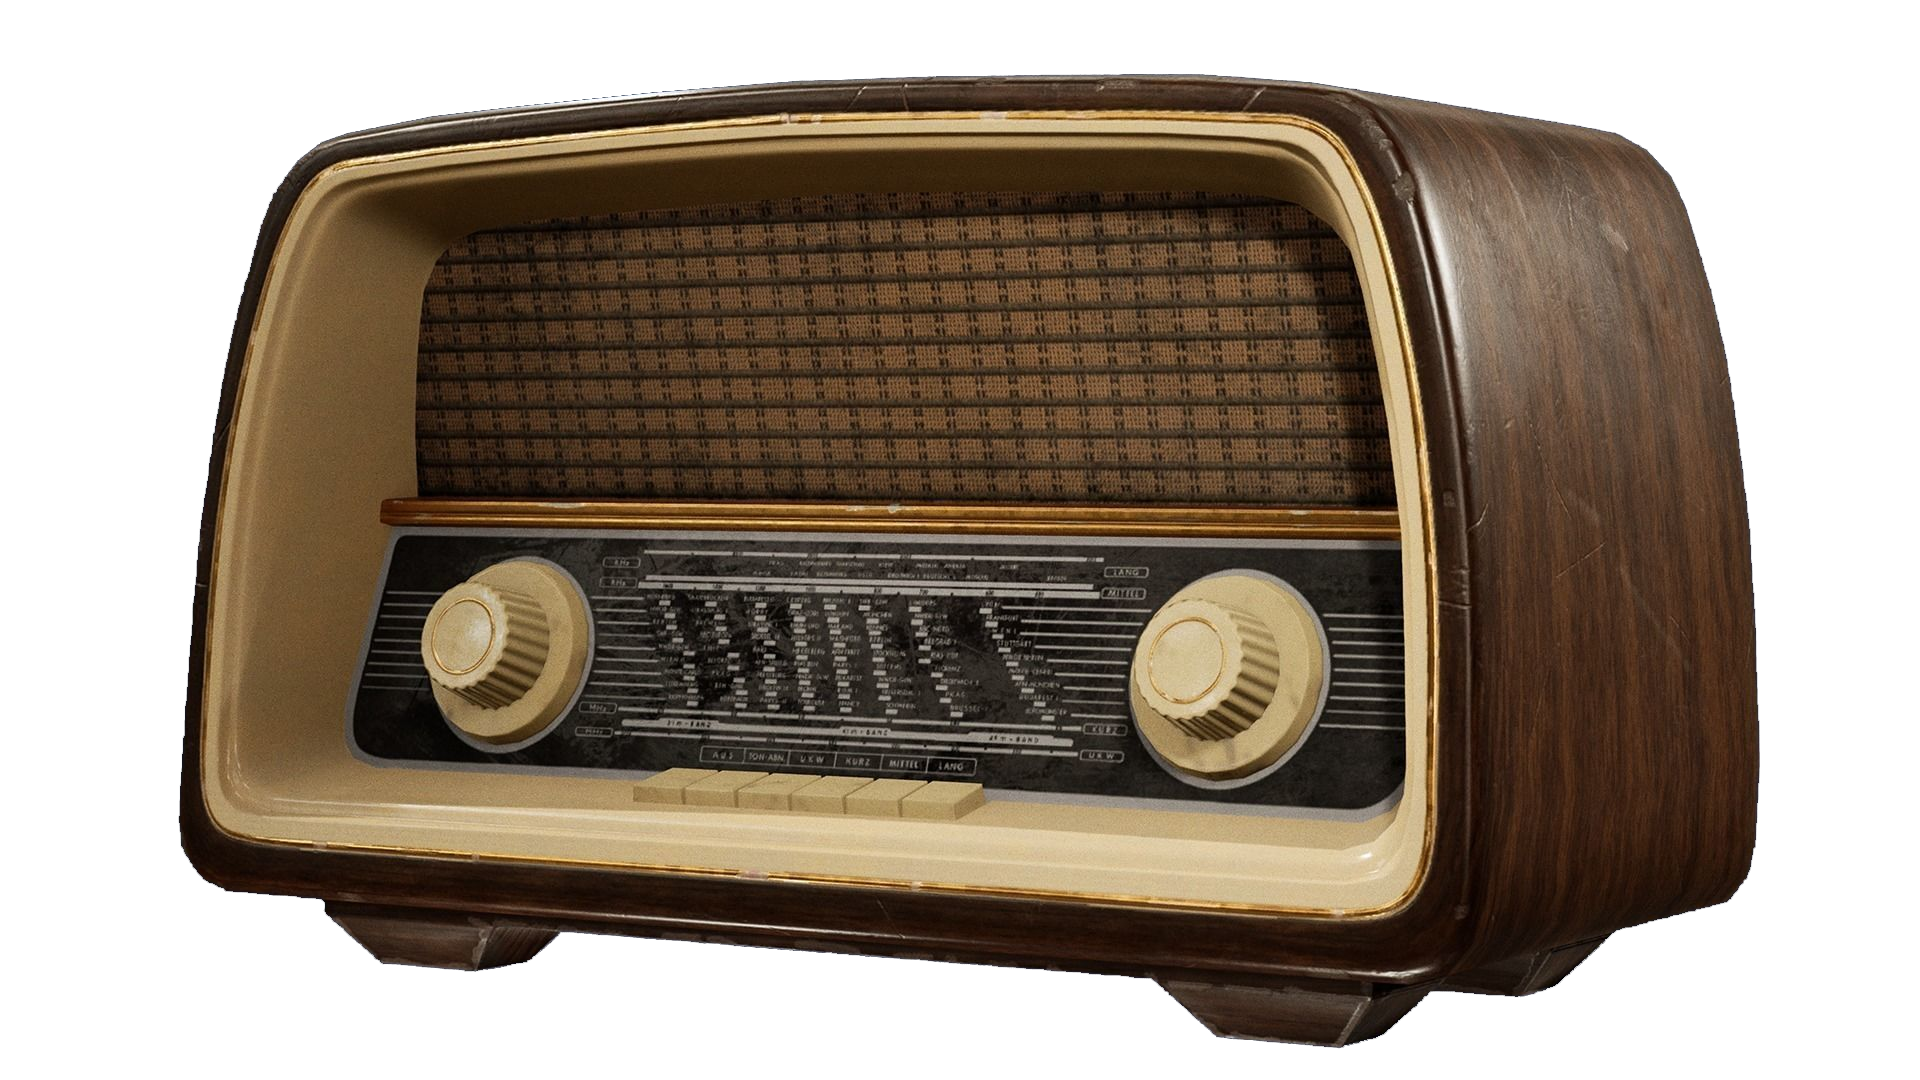
\includegraphics[width=1\linewidth]{img/assets/save.png}}
  \captionof{figure}{\emph{Borne de sauvegarde}}
  \label{fig:save}
\end{minipage}%
\end{figure}


\vfill
\noindent\makebox[\linewidth]{\rule{.8\paperwidth}{.6pt}}\\[0.2cm]
EPITA Toulouse - Projet S2 - 2022 \hfill Nyctalopia - gameHUB
\noindent\makebox[\linewidth]{\rule{.8\paperwidth}{.6pt}}

\subsection{Gameplay}
\setlength{\parindent}{5ex}
Concernant la partie jouable, nous avons tout d'abord appris à nous familiariser avec les différents outils mis à disposition par \emph{Unity3D} pour enregistrer les entrées du joueur, telles que les appuis sur les touches du clavier ou les mouvements de la souris.
Nous avons finalement choisi d'utiliser le \emph{New Input System}, qui nous permettrait par la suite de pouvoir implémenter des touches personnalisables, caractéristique que nous n'avons pas eu le temps d'implémenter.
\par
Par la suite nous avons donc crée le script responsable du mouvement de la caméra du joueur, celui-ci permet au joueur de déplacer la caméra dans la limite du physiquement possible par un humain, pour garder la sensation d'un jeu à la première personne dans lequel on incarne un humain. La caméra est donc bloquée à la verticale en haut et en bas, et les mouvements sur le côté tournent le corps du joueur.
\par
Le script permettant au joueur de se déplacer a été le suivant à être implémenté. Il permet au joueur de se déplacer avec quatre touches, lui servant à se déplacer vers l'avant, en arrière, à gauche et à droite.
Une touche permettant de s'accroupir, un \emph{RayCast} est utilisé pour savoir si le joueur peut se relever, si un objet ne se situe pas au-dessus de lui.
Enfin une touche pour courir à été ajoutée.
Nous avons décidé de ne pas implémenter d'action ''sauter'' pour limiter les déplacements du joueur et rendre le \emph{Gameplay} plus oppressant.
Pour les actions ''courir'' et ''s'acroupir'', un \emph{CallbackContext.performed} à été utilisé pour ne pas avoir à maintenir la touche enfoncée.

\vfill
\noindent\makebox[\linewidth]{\rule{.8\paperwidth}{.6pt}}\\[0.2cm]
EPITA Toulouse - Projet S2 - 2022 \hfill Nyctalopia - gameHUB
\noindent\makebox[\linewidth]{\rule{.8\paperwidth}{.6pt}}
\newpage

\par
Enfin, pour cette dernière soutenance, nous avons ajouté plusieurs scripts à notre projet:

\begin{figure}[H]
\centering
\begin{minipage}{.5\textwidth}
  \centering
  \centerline{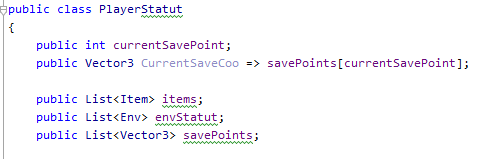
\includegraphics[width=1.5\linewidth]{img/gameplay/playerstatut.PNG}}
  \captionof{figure}{\emph{PlayerStatut}}
  \label{fig:octobercrowfont}
\end{minipage}%
\end{figure}

\begin{description}
  \item[\emph{PlayerStatut -}] une classe permettant de stocker l’avancée du joueur dans sa partie. Ce script permet de tenir à jour la réussite des différents puzzles et l’ouverture de différentes portes du jeu à travers la récupération des divers objets nécessaires à leur réussite ou leur ouverture. Ce script garde aussi en mémoire les coordonnées du dernier point de sauvegarde utilisé pour y placer le joueur lors de sa prochaine mort ou du prochain lancement de la partie.
  Pour réaliser se script, nous avons eu besoin de créer deux autres classes:
  \begin{description}
    \item[$\bullet$ \emph{Item} -] qui contient l’identifiant de l’objet
    \item[$\bullet$ \emph{Env} -] qui contient l’identifiant des portes et énigmes résolues par le joueur
\end{description}
\emph{PlayerStatut} stocke les différents éléments de \emph{Item} et \emph{Env} dans des listes.
Lors de l’ouverture d’une porte nous vérifions si l’\emph{Item} correspondant à la clé est bien dans le \emph{PlayerStatut} du joueur grâce à l'identifiant de l'objet et nous ajoutons cette porte à la liste d’\emph{Env}. Lors du prochain lancement de la partie, tous les \emph{GameObjet} possédant l'étiquette \emph{Door} serons récupérés et ceux ayant le même identifiant verrons leur script attaché à \emph{Interactable} exécuté, les portes serons donc ouvertes comme au moment de la sauvegarde, grâce à une méthode de la classe \emph{SaveManager}. Seulement les portes liées à des énigmes ou ouvertes grâce à une clé seront gardées en mémoires.
\end{description}

\vfill
\noindent\makebox[\linewidth]{\rule{.8\paperwidth}{.6pt}}\\[0.2cm]
EPITA Toulouse - Projet S2 - 2022 \hfill Nyctalopia - gameHUB
\noindent\makebox[\linewidth]{\rule{.8\paperwidth}{.6pt}}
\newpage

\begin{figure}[H]
\centering
\begin{minipage}{.5\textwidth}
  \centering
  \centerline{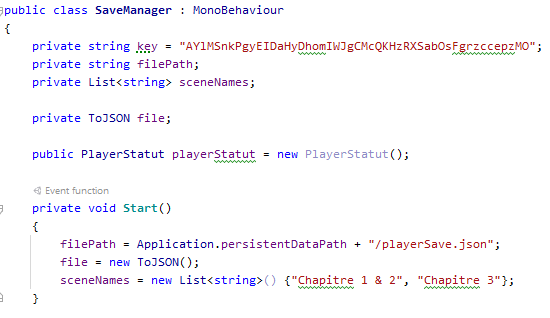
\includegraphics[width=1.5\linewidth]{img/gameplay/Savamanager.PNG}}
  \captionof{figure}{\emph{SaveManager}}
  \label{fig:octobercrowfont}
\end{minipage}%
\end{figure}

\begin{description}
  \item[\emph{SaveManager -}] un script lié aux bornes de sauvegarde disséminées à des endroits prédéfinis dans le jeu. Cette classe possède le \emph{PlayerStatut} actuel, le chemin d'accès pour accéder au fichier de sauvegarde récupéré grâce au \emph{Application.persistentPath} mis à disposition par \emph{Unity3D}. Celle-ci possède aussi le nom des différentes scènes utilisées.
  \newline
  De plus, une instance de la classe \emph{ToJSON} est présente dans la classe, permettant de garder en mémoire les sauvegardes, cette classe sera ensuite sérialisée dans le format JSON (1) et chiffrées grâce au chiffrage XOR (XOR Cipher) (2), empêchant ainsi le joueur de tricher en modifiant sa sauvegarde.
  De plus, cette classe possède différentes méthodes permettant d'ajouter des \emph{Item} et des \emph{Env} mais aussi de vérifier si un \emph{Item} est possédé ou si un \emph{Env} à été complété.
  Comme évoqué dans la description de la classe \emph{PlayerStatut}, la méthode \emph{Refresh} recharge la scène de la dernière sauvegarde, donne les items que possédait le joueur lors de la sauvegarde et ouvre les portes gardées en mémoire.
\end{description}
 
 
\vfill
\noindent\makebox[\linewidth]{\rule{.8\paperwidth}{.6pt}}\\[0.2cm]
EPITA Toulouse - Projet S2 - 2022 \hfill Nyctalopia - gameHUB
\noindent\makebox[\linewidth]{\rule{.8\paperwidth}{.6pt}}

\newpage

\begin{figure}[H]
\centering
\begin{minipage}{.5\textwidth}
  \centering
  \centerline{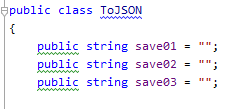
\includegraphics[width=1.5\linewidth]{img/gameplay/tojson.PNG}}
  \captionof{figure}{\emph{ToJSON}}
  \label{fig:octobercrowfont}
\end{minipage}%
\end{figure}
 
  \begin{description}
 \item[\emph{ToJSON -}] Cette classe contient les trois emplacements de sauvegarde sous forme de chaîne de caractères au format JSON pour empêcher tout problème de référence.
 C'est cette classe qui sera transformée en fichier de sauvegarde.
\end{description}

\begin{description}
    \item[(1) :] Le format JSON (JavaScript Object Notation) est un format couramment utilisé pour représenter de l’information structurée sous forme de texte. Il est facilement lisible par des humains (malgré le manque d’espaces nécessaire pour alléger le fichier).
    \begin{figure}[H]
        \centering
        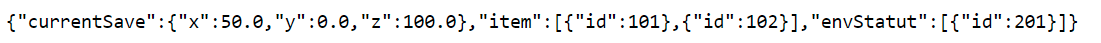
\includegraphics[width=18cm]{img/gameplay/JSONRaw.PNG}
        \caption{ Fichier JSON}
        \label{fig:JSONraw}
    \end{figure}
    
    \item[(2) :] Le chiffrage XOR utilise l’opérateur binaire XOR (OU-exclusif), voici sa table de vérité:
    \newline
    \begin{figure}[H]
        \centering
        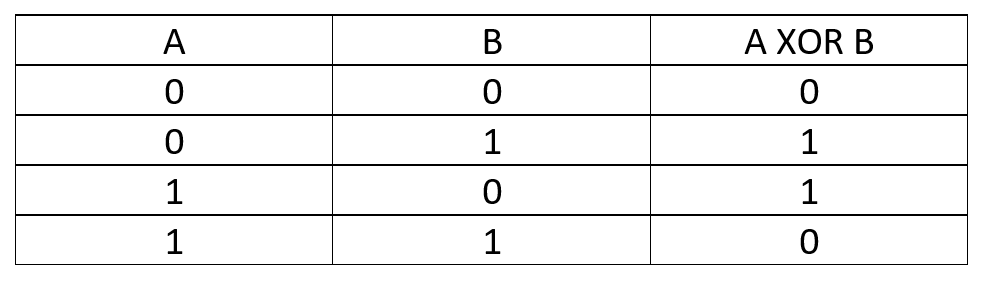
\includegraphics[width=10cm]{img/gameplay/XORtable.PNG}
        \caption{ Table de vérité OU-exclusif}
        \label{fig:XORtable}
    \end{figure}
\end{description}
\par

    
    
\vfill
\noindent\makebox[\linewidth]{\rule{.8\paperwidth}{.6pt}}\\[0.2cm]
EPITA Toulouse - Projet S2 - 2022 \hfill Nyctalopia - gameHUB
\noindent\makebox[\linewidth]{\rule{.8\paperwidth}{.6pt}}
\newpage

Lors du chiffrage nous allons passer à travers une porte logique XOR chaque lettre de nôtre chaîne de caractères avec la lettre au même indice, le tout modulo la longueur de notre clé, et ainsi reconstruire une chaîne de caractères chiffrée, de même longueur mais inintelligible.
Lors du déchiffrement nous allons effectuer les mêmes actions mais avec la chaîne de caractères chiffrée à la place de celle en claire.
Pour passer deux lettres à travers la porte XOR on passe en réalité les représentations binaires des codes ASCII (American Standard Code for Information Interchange) de ces lettres, le résultat sera donc une représentation binaire convertie en nombre et retranscrite grâce à la table ASCII.
Exemple : 
Dans cet exemple on souhaite chiffrer le mot ''MESSAGE'' avec la clé ''CLE'' :

    \begin{figure}[H]
        \centering
        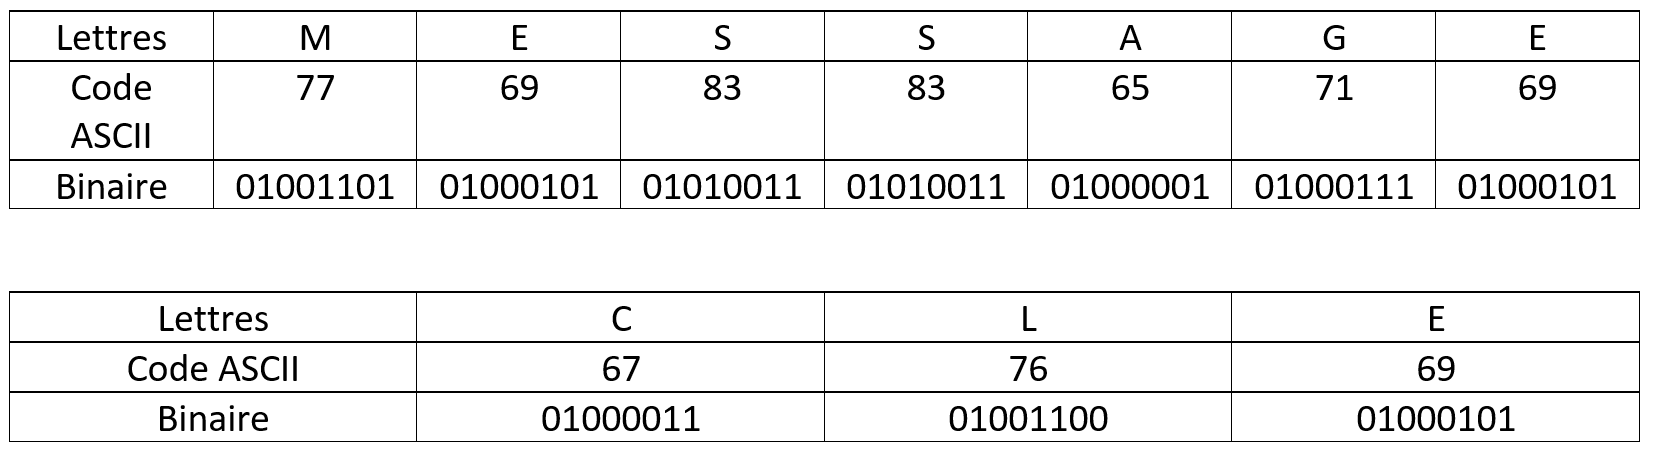
\includegraphics[width=15cm]{img/gameplay/clemsgtranscript.PNG}
        \caption{ Conversion des lettres en binaire}
        \label{fig:transciption}
    \end{figure}
    
Le chiffrement XOR va donc correspondre à ceci :
 \newline
    \begin{figure}[H]
        \centering
        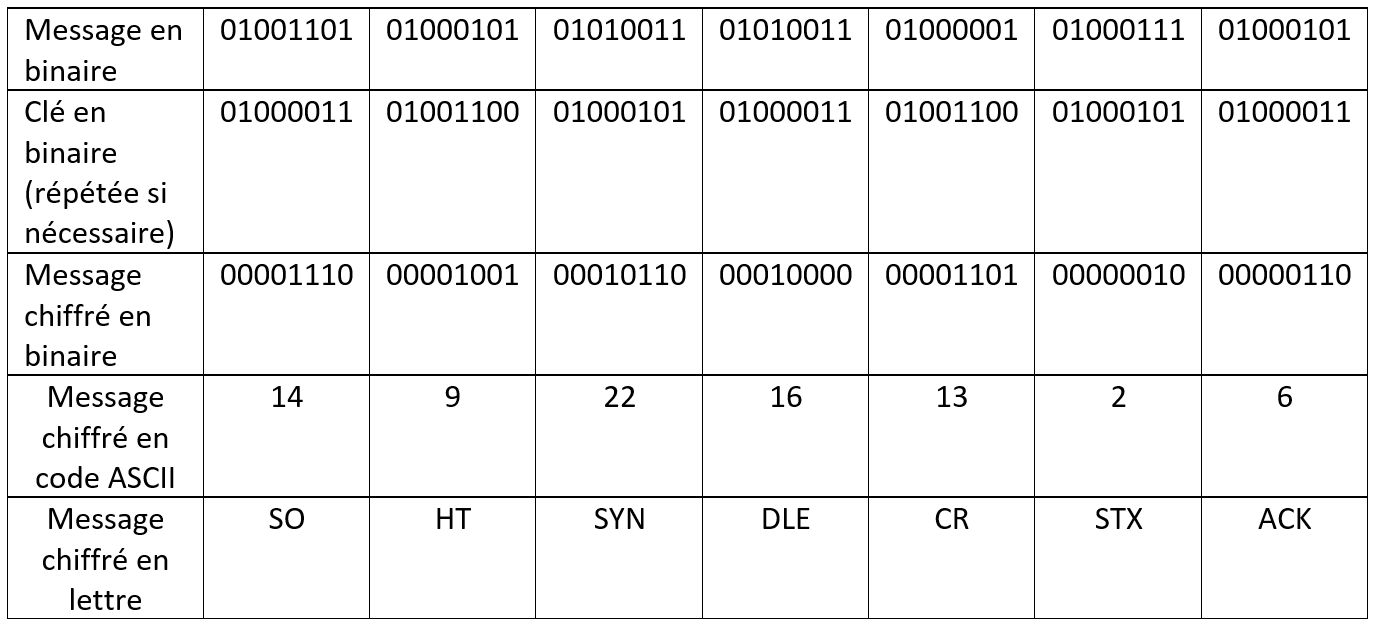
\includegraphics[width=17cm]{img/gameplay/Xorencryot.PNG}
        \caption{ Conversion des lettres en binaire}
        \label{fig:XORencryption}
    \end{figure}

    
    
\vfill
\noindent\makebox[\linewidth]{\rule{.8\paperwidth}{.6pt}}\\[0.2cm]
EPITA Toulouse - Projet S2 - 2022 \hfill Nyctalopia - gameHUB
\noindent\makebox[\linewidth]{\rule{.8\paperwidth}{.6pt}}
\newpage

Dans cet exemple le message chiffré est composé uniquement de caractères ASCII non imprimables et de caractères de contrôle, utilisés pour contrôler certains périphériques ou donner des indications sur le format du document.
\newline
Le chiffrement XOR est basique et le message chiffré peut être facilement décrypté si la clé est trop petite par rapport à la taille du message grâce à une analyse fréquentielle ou dans ce cas d’utilisation (sauvegarde), par une attaque à texte clair connu étant donné que le joueur connaît les noms des objets.
\newline
Nous avons choisi de créer une clé de 50 caractères choisis aléatoirement parmi les caractères dits imprimables de la table ASCII.
Il est donc ici préférable de se référer aux objets par des nombres plutôt que des noms, nous choisissons de représenter les objets, les portes et énigmes réussis par des identifiants.
Pour un souci de lisibilité nous avons aussi ajouté un dictionnaire liant les identifiants des objets, portes et énigmes à leurs noms.
\newline
De plus, pour l’instant, la clé de chiffrement est unique pour toutes les sauvegardes et tous les joueurs mais il peut être intéressant d’en générer une nouvelle aléatoirement à chaque création d’une nouvelle partie en retranscrivant ce code en C\#.

Nous avons aussi implémenté la touche ''utiliser'' assignée à la touche ''E''. Nous utiliserons le système de \emph{RayCast} (qui peut être traduit par ‘’lancé de rayon’’) et le système \emph{Event} proposé par Unity3D pour découper ce système en deux scripts distincts: \emph{Interactor} et \emph{Interactable}. Ils seront respectivement liés au joueur et aux objets que l’on veut interactifs tels que les bornes de sauvegarde, les puzzles, les clés à récupérer, les portes…

    
    
\vfill
\noindent\makebox[\linewidth]{\rule{.8\paperwidth}{.6pt}}\\[0.2cm]
EPITA Toulouse - Projet S2 - 2022 \hfill Nyctalopia - gameHUB
\noindent\makebox[\linewidth]{\rule{.8\paperwidth}{.6pt}}
\newpage


\newline
\begin{description}
    \begin{figure}[H]
\centering
\begin{minipage}{.5\textwidth}
  \centering
  \centerline{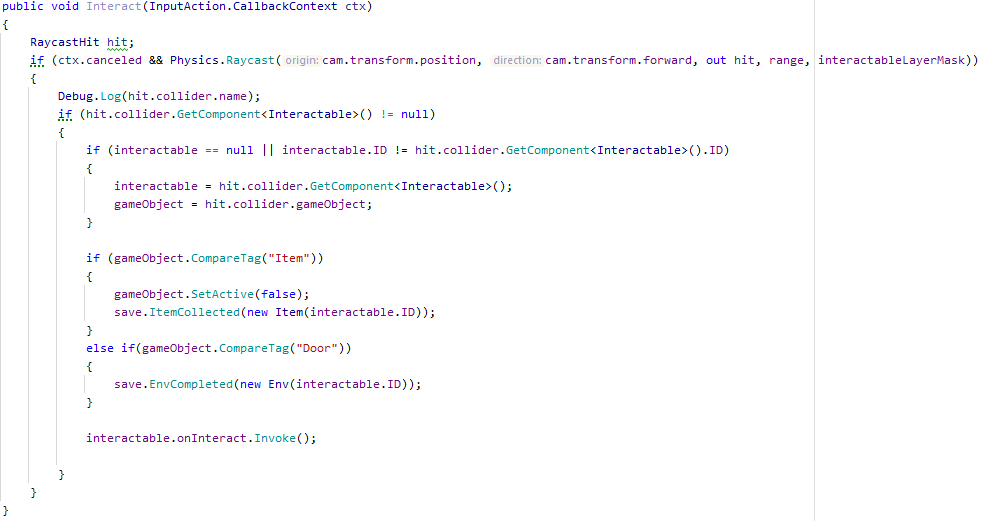
\includegraphics[width=2.25\linewidth]{img/gameplay/interactor.PNG}}
  \captionof{figure}{\emph{Interactor}}
  \label{fig:octobercrowfont}
\end{minipage}%
\end{figure}
    \item[\emph{Interactor} -] Ce script est lié au joueur et permet grâce au \emph{Raycasting} de savoir si le joueur pointe son curseur vers un objet possèdant la couche \emph{Interactable} et si celui-ci est assez proche du joueur. Ensuite nous récupérons le \emph{GameObject} et nous lançons la fonction liée à l’objet à travers le script \emph{Interactable}. De plus, si l’objet possède l'étiquette \emph{Item}, celui-ci sera ajouté à l’inventaire du joueur et sera désactivé pour le faire disparaître, d’autre part, si l’objet possède l'étiquette \emph{Door}, cette porte sera gardée en mémoire et sera ouverte lorsque le joueur chargera sa sauvegarde. Cette fonction est appelée quand le joueur appuie sur la touche ''E''.
\begin{figure}[H]
\centering
\begin{minipage}{.5\textwidth}
  \centering
  \centerline{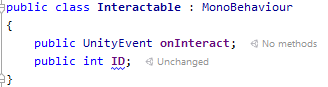
\includegraphics[width=1.5\linewidth]{img/gameplay/interactable.PNG}}
  \captionof{figure}{\emph{Interactable}}
  \label{fig:octobercrowfont}
\end{minipage}%
\end{figure}
    \item[\emph{Interactable} -] Ce script est lié à l’objet avec lequel nous voulons interagir, il est composé d’un identifiant et d’un \emph{UnityEvent} permettant d’appeler une fonction.
\end{description}

   
\vfill
\noindent\makebox[\linewidth]{\rule{.8\paperwidth}{.6pt}}\\[0.2cm]
EPITA Toulouse - Projet S2 - 2022 \hfill Nyctalopia - gameHUB
\noindent\makebox[\linewidth]{\rule{.8\paperwidth}{.6pt}}
\newpage


\par

Par la suite, nous avons implémenté la classe permettant d'activer/désactiver la lampe torche.
\begin{description}
\begin{figure}[H]
\centering
\begin{minipage}{.5\textwidth}
  \centering
  \centerline{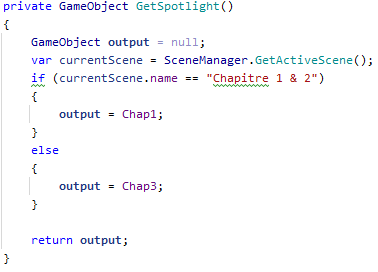
\includegraphics[width=1.5\linewidth]{img/gameplay/getspotlight.PNG}}
  \captionof{figure}{\emph{GetSpotlight}}
  \label{fig:octobercrowfont}
\end{minipage}%
\end{figure}
    \item[\emph{} GetSpotlight-] Ce script permet de récupérer le \emph{GameObject} qui représente le \emph{SpotLight} (Point Lumineux) représentant la lumière de la lampe torche, dans les chapitres 1 et 2 l’intensité de la lampe torche est moindre que celle du Chapitre 3, en effet le Chapitre 3 se situant dans un endroit clos il est nécessaire d’augmenter l’intensité pour pouvoir y voir correctement. Pour savoir quel \emph{GameObjet} nous devons utiliser, nous utilisons le \emph{SceneManager} mis à disposition par \emph{Unity3D} pour pouvoir connaître la Scène actuellement utilisée.

\vfill
\noindent\makebox[\linewidth]{\rule{.8\paperwidth}{.6pt}}\\[0.2cm]
EPITA Toulouse - Projet S2 - 2022 \hfill Nyctalopia - gameHUB
\noindent\makebox[\linewidth]{\rule{.8\paperwidth}{.6pt}}
\newpage
    
    \begin{figure}[H]
\centering
\begin{minipage}{.5\textwidth}
  \centering
  \centerline{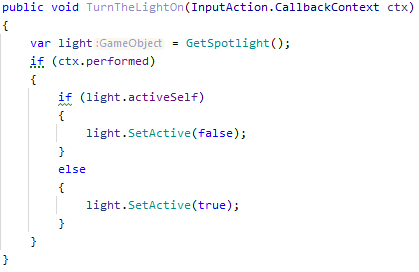
\includegraphics[width=1.2\linewidth]{img/gameplay/turnthelighton.PNG}}
  \captionof{figure}{\emph{TurnTheLightOn}}
  \label{fig:octobercrowfont}
\end{minipage}%
\end{figure}
    \item[\emph{} TurnTheLightOn-] Ce script permet d’éteindre et d’allumer la lampe torche, l’utilisation du \emph{ctx.performed} permet de basculer d’un état à l’autre avec un simple appui sur la touche prévue à cet effet, le \emph{Unity Input System} permet d’appeler cette fonction lorsque la touche ''T'' est appuyée.
\end{description}

\vspace*{7mm}

\par

Nous avons enfin implémenté \emph{DevMod} permettant de lancer le jeu en mode Développeur. Cette fonction permet de charger la scène suivante à celle dans laquelle se trouve le joueur.

\vfill
\noindent\makebox[\linewidth]{\rule{.8\paperwidth}{.6pt}}\\[0.2cm]
EPITA Toulouse - Projet S2 - 2022 \hfill Nyctalopia - gameHUB
\noindent\makebox[\linewidth]{\rule{.8\paperwidth}{.6pt}}
\newpage

\subsection{Communication}
\setlength{\parindent}{5ex}

Le logo Nyctalopia, après plusieurs étapes de conception, est écrit en noir avec la police \emph{October Crow} et se présente dans le menu principal du jeu ainsi qu'à la fin de la cinématique de début de jeu.

\begin{figure}[H]
\centering
\begin{minipage}{.5\textwidth}
  \centering
  \centerline{
\includegraphics[width=1\linewidth]{img/font.png}}
  \captionof{figure}{\emph{Police d'écriture choisie pour Nyctalopia}}
  \label{fig:octobercrowfont}
\end{minipage}%
\end{figure}

Concernant le logo du studio, que nous avons réussit à le désigner assez rapidement, nous nous sommes inspirés du logo de \emph{GitHub}, comme peut en témoigner le nom de notre studio.


\begin{figure}[H]
\centering
\begin{minipage}{.5\textwidth}
  \centering
  \centerline{
\includegraphics[width=1\linewidth]{img/logos/logo.png}}
  \captionof{figure}{\emph{Logo choisi pour GameHub Studio}}
  \label{fig:octobercrowfont}
\end{minipage}%
\end{figure}


\vfill
\noindent\makebox[\linewidth]{\rule{.8\paperwidth}{.6pt}}\\[0.2cm]
EPITA Toulouse - Projet S2 - 2022 \hfill Nyctalopia - gameHUB
\noindent\makebox[\linewidth]{\rule{.8\paperwidth}{.6pt}}
\newpage


Enfin, pour le logo du jeu, nous avons eu plus de mal à trouver un logo convenable et esthétique pour pouvoir correspondre à une icône Windows, ou une icône de jeu Steam. Finalement nous avons opté pour un logo simple avec l'initiale du nom du jeu dans un hexagone légèrement stylisé avec un effet de lunettes 3D rouge/bleu.

\vspace*{7mm}
\begin{figure}[H]
\centering
\begin{minipage}{.5\textwidth}
  \centering
  \centerline{
\includegraphics[width=1\linewidth]{img/logos/logojeu.png}}
  \captionof{figure}{\emph{Icône du jeu}}
  \label{fig:octobercrowfont}
\end{minipage}%
\end{figure}


\vfill
\noindent\makebox[\linewidth]{\rule{.8\paperwidth}{.6pt}}\\[0.2cm]
EPITA Toulouse - Projet S2 - 2022 \hfill Nyctalopia - gameHUB
\noindent\makebox[\linewidth]{\rule{.8\paperwidth}{.6pt}}
\newpage


\subsection{Graphismes, Modèles et Terrain}
\setlength{\parindent}{5ex}

\emph{Nyctalopia} suit un sytème de chapitres. Lors du parcours de chacun des 3 chapitres crées, le joueur retrouvera une zone caractéristique représentant le chapitre. A savoir: la forêt, la base militaire et les égouts. Lors du début de la partie, le joueur retrouve une cinématique d'une minute trente secondes, où le joueur est introduit au monde de \emph{Nyctalopia} et est mis en contexte de l'histoire qui commence par un accident de voiture.

\begin{figure}[H]
\centering
\begin{minipage}{.5\textwidth}
  \centering
  \centerline{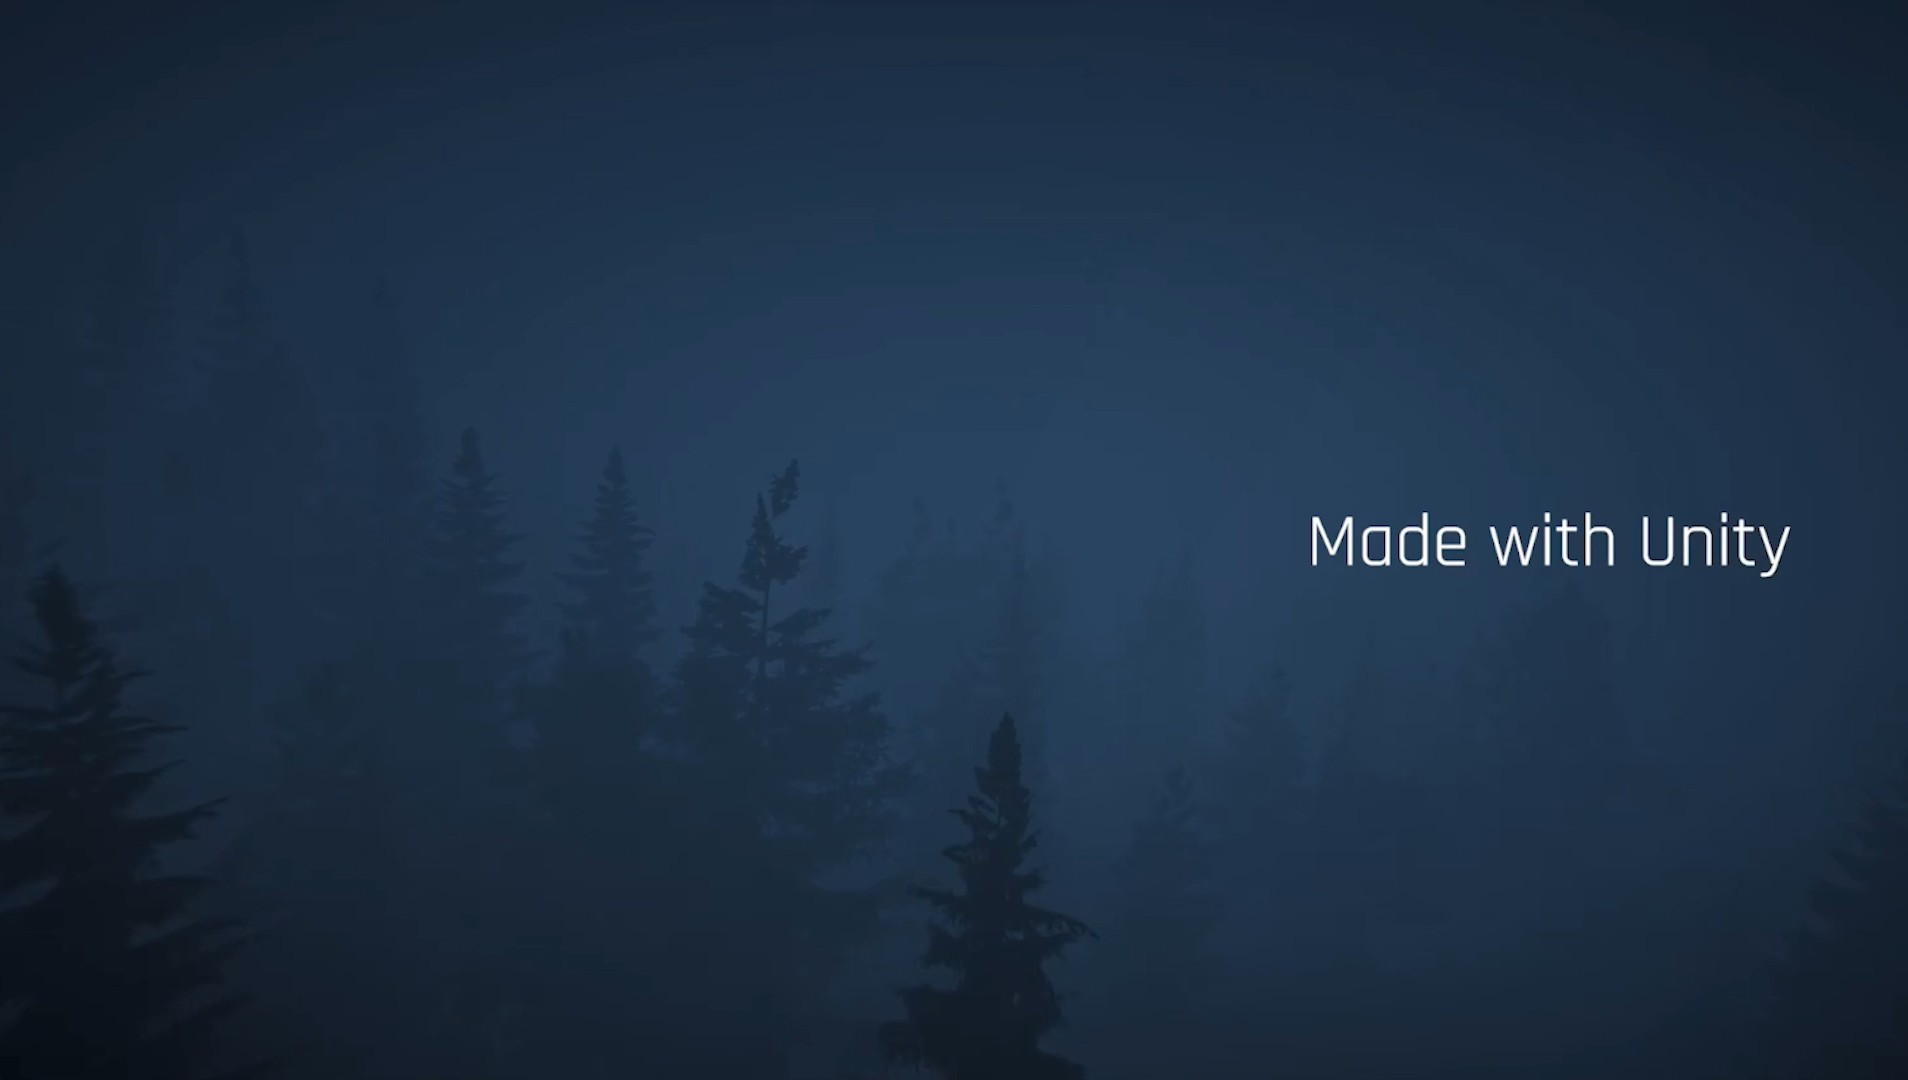
\includegraphics[width=1\linewidth]{img/cine.png}}
  \captionof{figure}{\emph{Prologue}}
  \label{fig:cinematique}
\end{minipage}%
\end{figure}

Le chapitre 1 se passe dans une forêt. Une grande variété de modèles 3D d’arbres, arbustes et herbe ont été sélectionnés et utilisés dans le jeu pour couvrir ce terrain et créer une forêt riche et variée. La plupart de ces modèles de végétation proviennent de la bibliothèque de modèles 3D \emph{Quixel’s Megascans} et du site officiel de modèles Unity: \emph{Unity Asset Store}. Plusieurs modifications et conversions ont été nécessaires pour les rendre compatibles avec notre projet qui est basé sur le système de rendu HDRP (\emph{High-Definition Render Pipeline}) qui offre des résultats graphiques plus attractifs.
\newline

\begin{figure}[H]
\centering
\begin{minipage}{.5\textwidth}
  \centering
  \centerline{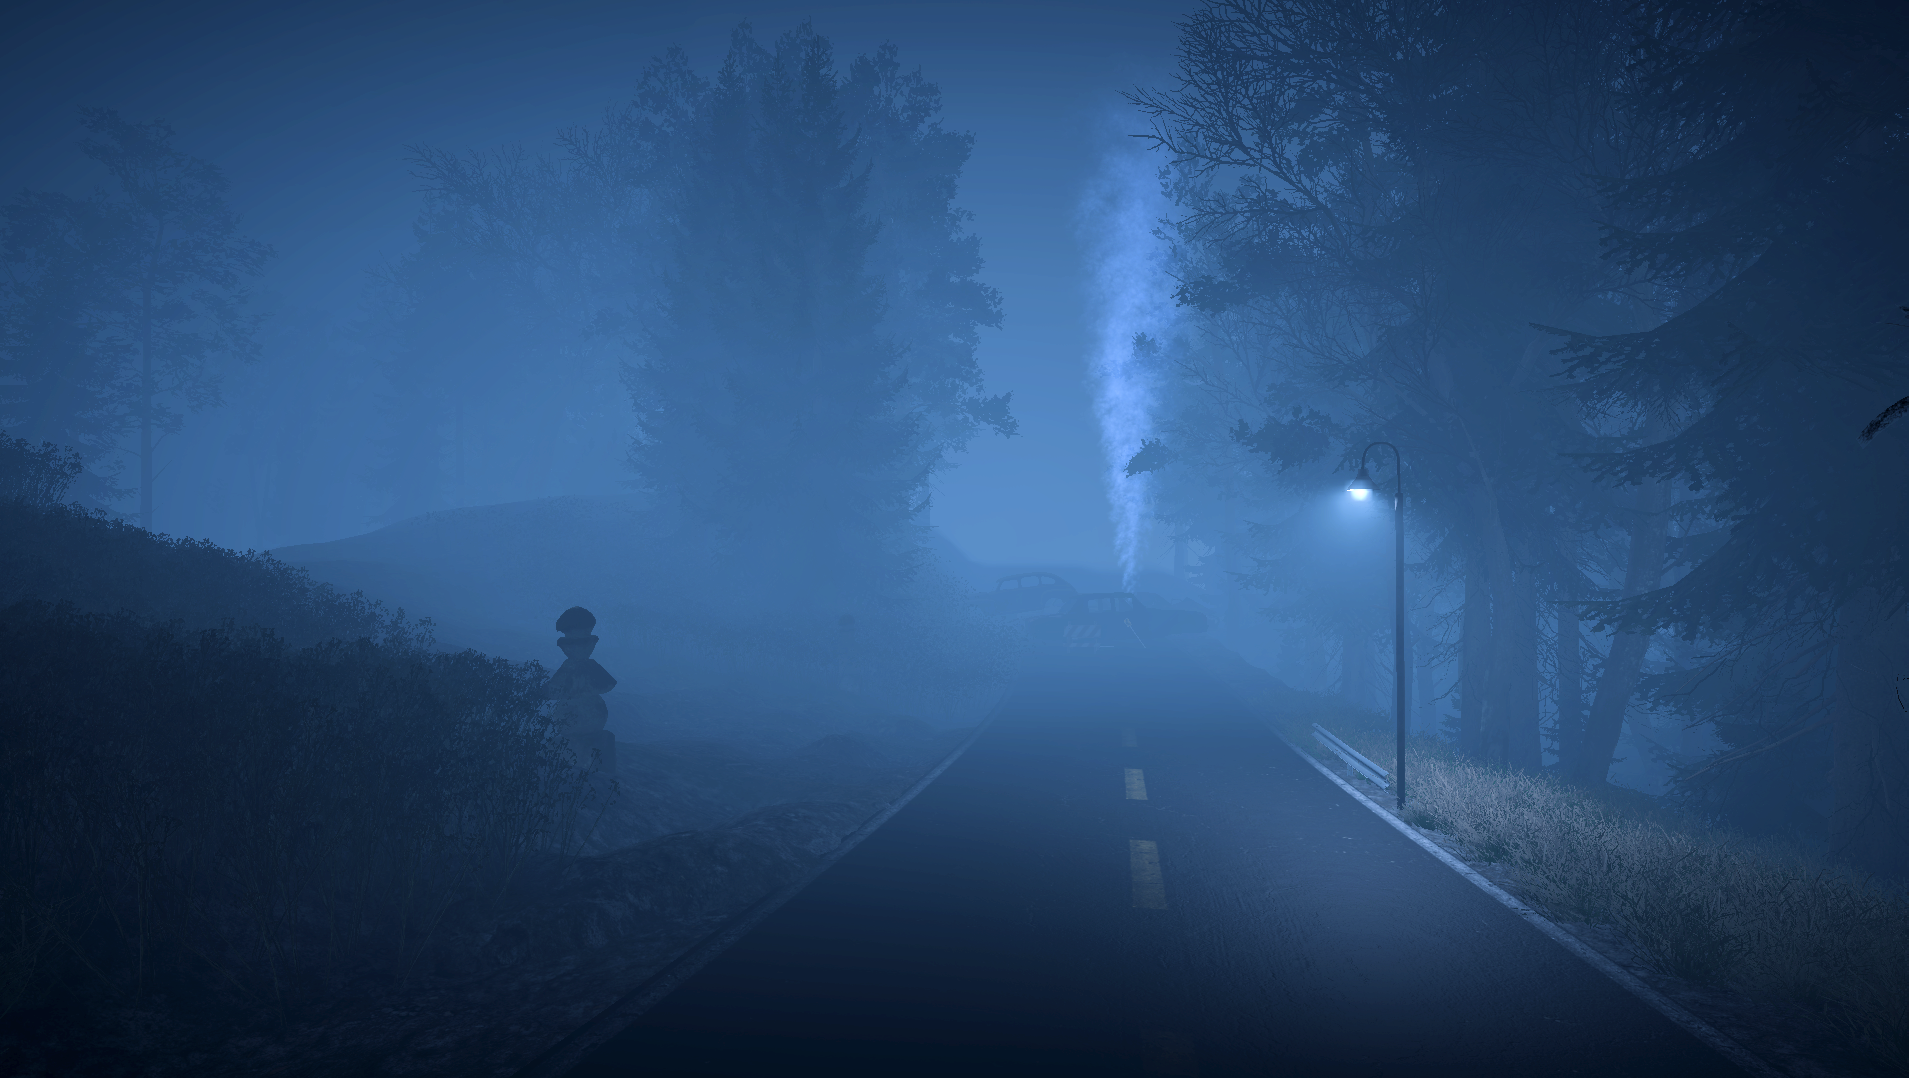
\includegraphics[width=1\linewidth]{img/uwufolder/spawn.png}}
  \captionof{figure}{\emph{Chapitre 1}}
  \label{fig:cinematique}
\end{minipage}%
\end{figure}


\vfill
\noindent\makebox[\linewidth]{\rule{.8\paperwidth}{.6pt}}\\[0.2cm]
EPITA Toulouse - Projet S2 - 2022 \hfill Nyctalopia - gameHUB
\noindent\makebox[\linewidth]{\rule{.8\paperwidth}{.6pt}}
\newpage

Le chapitre 2 se passe dans une base militaire. Une grande variété de modèles 3D d’arbres, arbustes et herbe ont été sélectionnés et utilisés dans le jeu pour couvrir ce terrain et créer une forêt riche et variée. La plupart de ces modèles de végétation proviennent de la bibliothèque de modèles 3D \emph{Quixel’s Megascans} et du site officiel de modèles Unity: \emph{Unity Asset Store}. Plusieurs modifications et conversions ont été nécessaires pour les rendre compatibles avec notre projet qui est basé sur le système de rendu HDRP (\emph{High-Definition Render Pipeline}) qui offre des résultats graphiques plus attractifs.
\newline

\begin{figure}[H]
\centering
\begin{minipage}{.5\textwidth}
  \centering
  \centerline{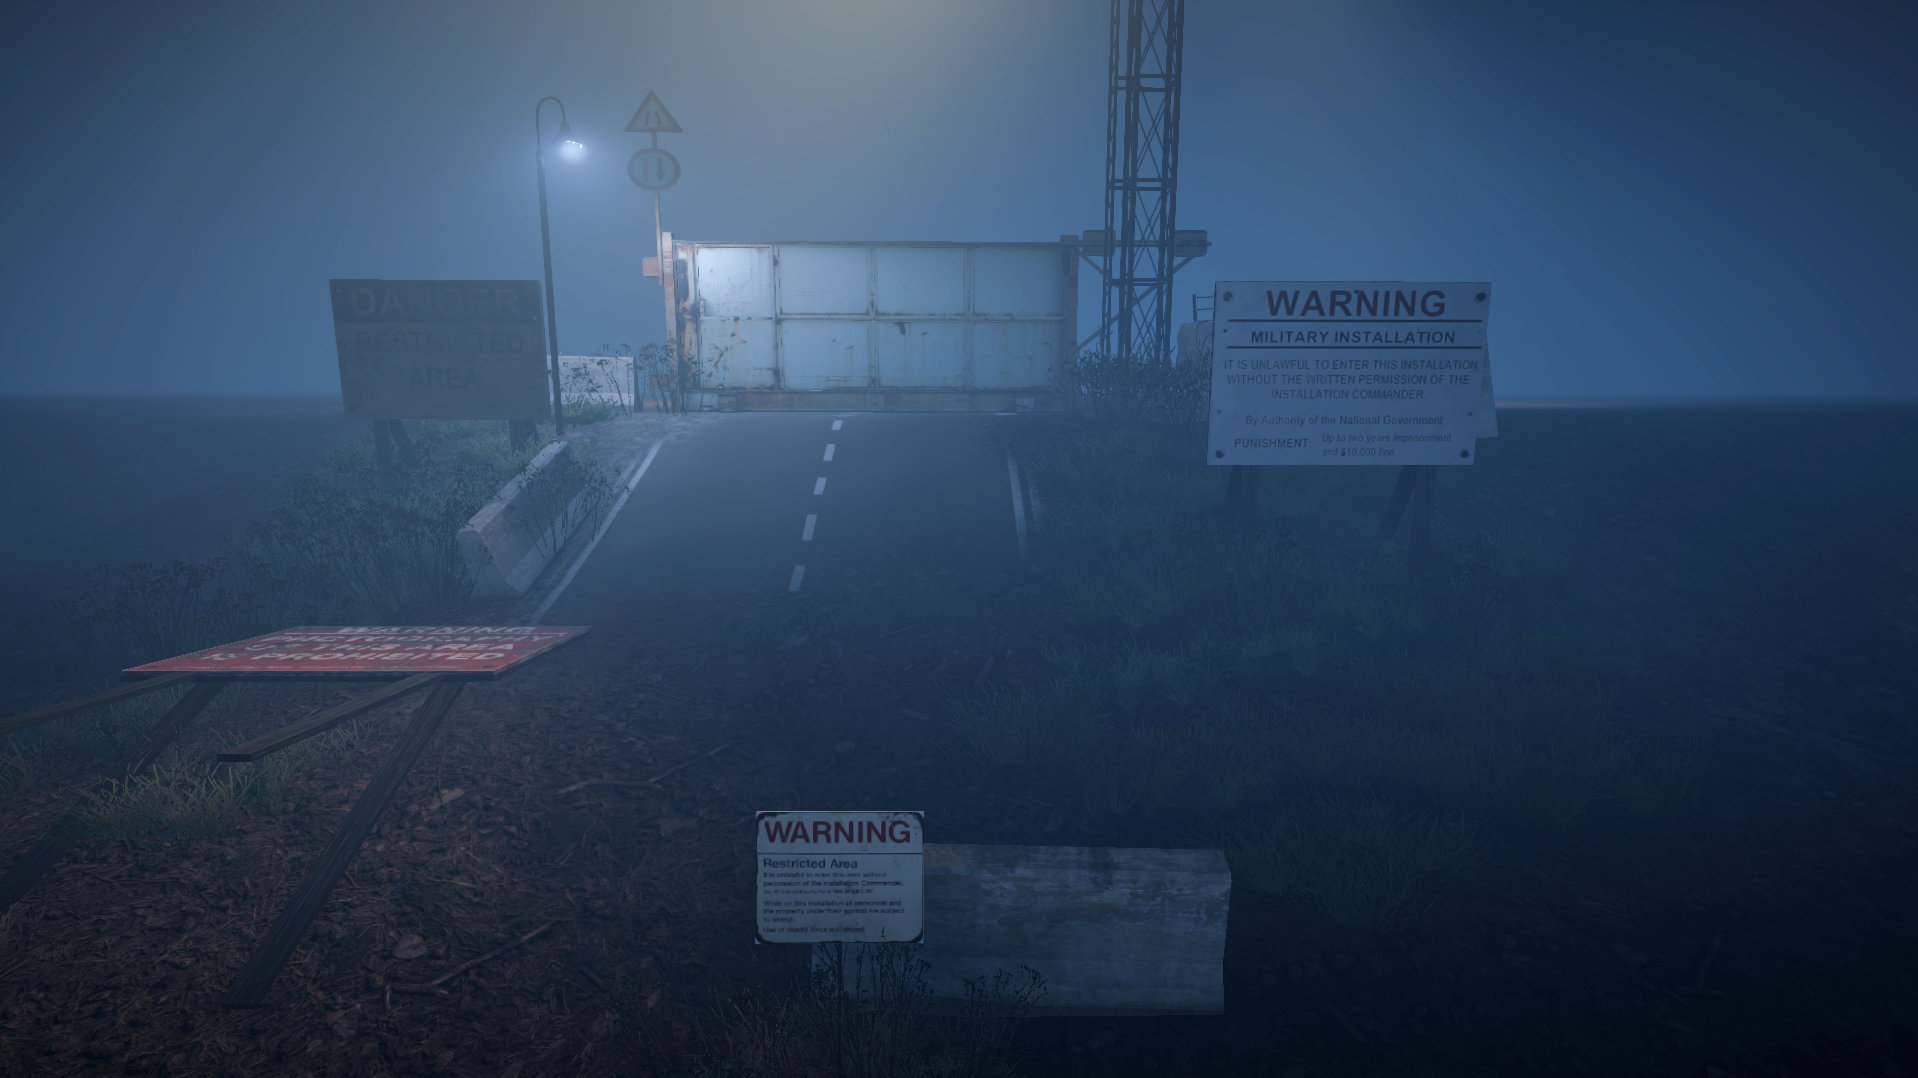
\includegraphics[width=1\linewidth]{img/uwufolder/military.png}}
  \captionof{figure}{\emph{Chapitre 2}}
  \label{fig:cinematique}
\end{minipage}%
\end{figure}

Enfin, le chapitre 3, se passe dans des égouts. L'utilisation de modèles 3D modulaires conçus pour la création d'égouts nous ont permis d'avoir le système souterrain désiré. 
\newline


\begin{figure}[H]
\centering
\begin{minipage}{.5\textwidth}
  \centering
  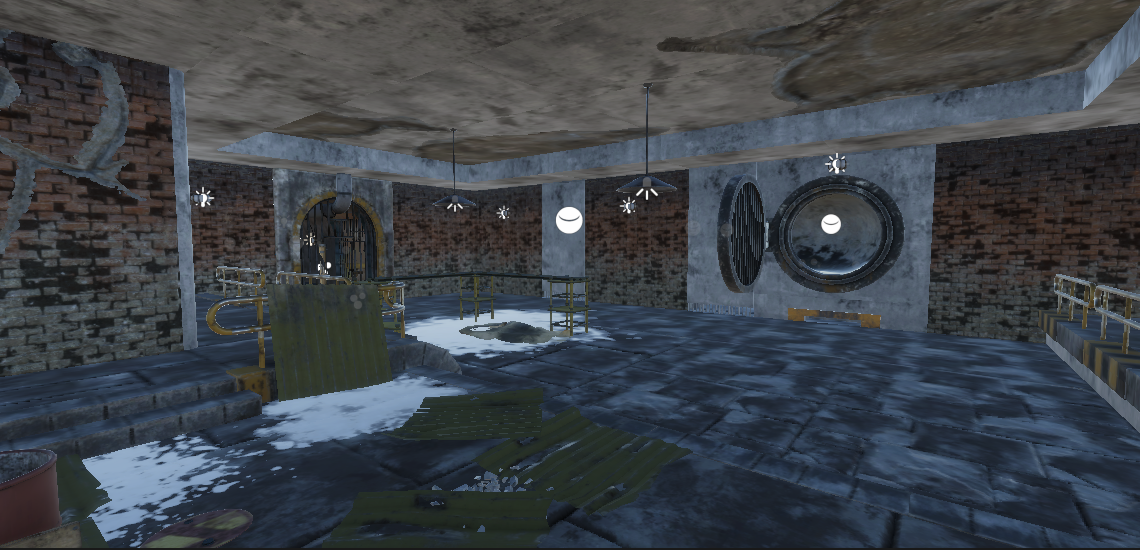
\includegraphics[width=.8\linewidth]{img/egouts/1.PNG}
  \captionof{figure}{\emph{Chapitre 3 - Les égouts}}
  \label{fig:chap3}
\end{minipage}%
\begin{minipage}{.5\textwidth}
  \centering
  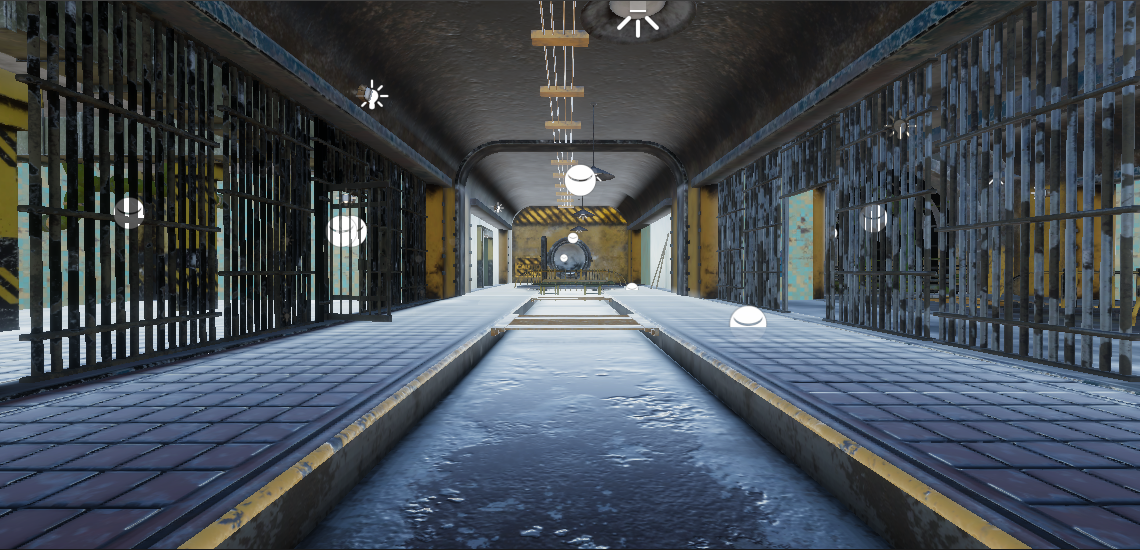
\includegraphics[width=.8\linewidth]{img/egouts/3.png}
  \captionof{figure}{\emph{Chapitre 3 - Les égouts}}
  \label{fig:chap3bis}
\end{minipage}
\end{figure}

\vfill
\noindent\makebox[\linewidth]{\rule{.8\paperwidth}{.6pt}}\\[0.2cm]
EPITA Toulouse - Projet S2 - 2022 \hfill Nyctalopia - gameHUB
\noindent\makebox[\linewidth]{\rule{.8\paperwidth}{.6pt}}
\newpage

Dans ce chapitre, le joueur retrouve une nouvelle mécanique de jeu: les leviers. Ces leviers après activation, ouvrent des portes dans le chapitre 3. La porte ouverte peut être déduite grâce au son 3D que les portes produisent dès que le joueur active ses leviers correspondants. Les leviers possèdent aussi un indicateur LED qui indique l'état du levier (désactivé, rouge clignotant/activé, vert).
Pour reconnaître que le joueur a utilisé la touche \emph{Action} sur eux, ils utilisent le script \emph{Interactable} qui va ensuite lancer le script \emph{LeverPress} mentionnés précédemment.
\newline

\begin{figure}[H]
\centering
\begin{minipage}{.5\textwidth}
  \centering
  \centerline{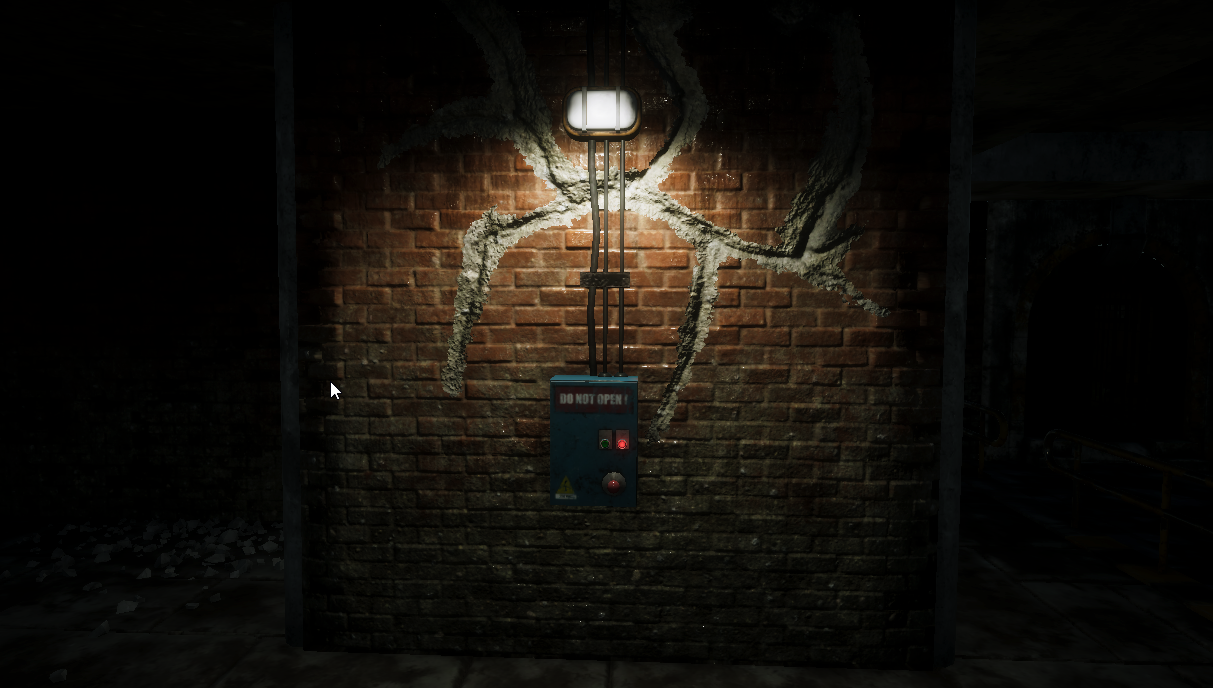
\includegraphics[width=1\linewidth]{img/uwufolder/bornes.png}}
  \captionof{figure}{\emph{Chapitre }}
  \label{fig:cinematique}
\end{minipage}%
\end{figure}

Dans ce chapitre le joueur pourra utiliser aussi une lampe torche pour se guider dans l'obscurité de ce chapitre. Cette lampe torche peut être allumée avec la touche associée à celle-ci (Par défaut, \textbf{T}).


\begin{figure}[H]
\centering
\begin{minipage}{.5\textwidth}
  \centering
  \centerline{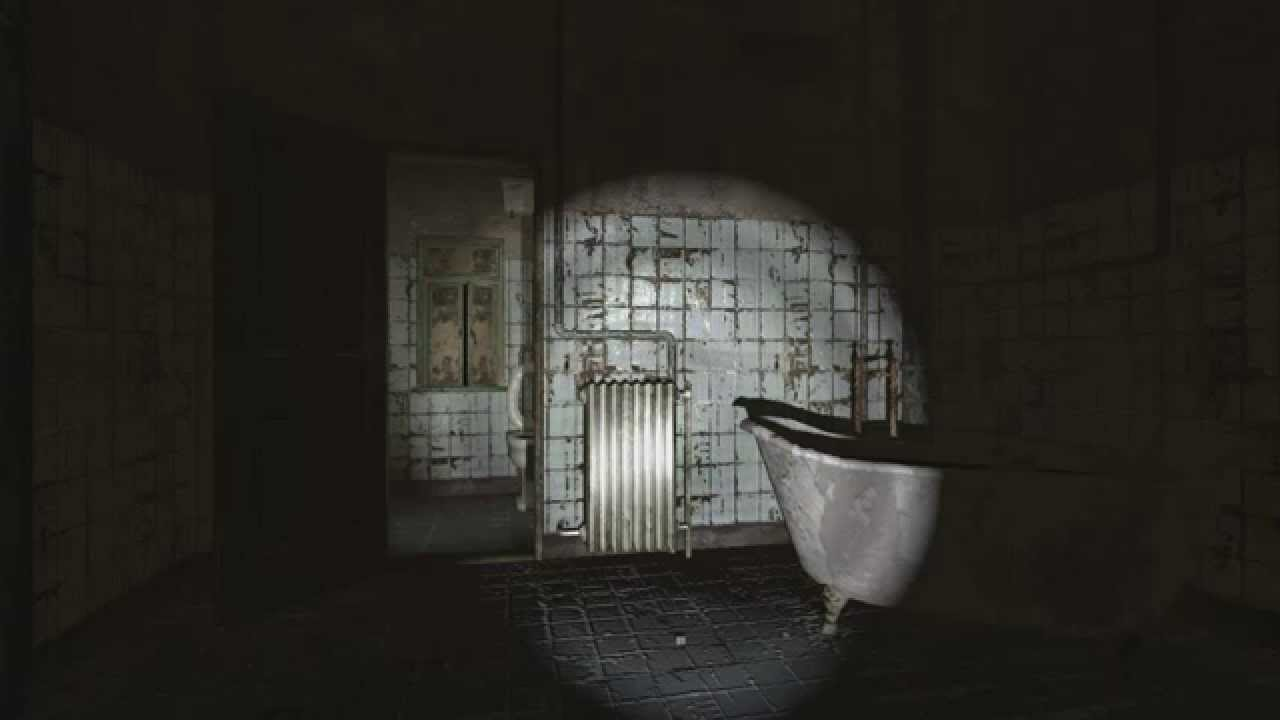
\includegraphics[width=1\linewidth]{img/egouts/light.jpg}}
  \captionof{figure}{\emph{Système de lampe torche}}
  \label{fig:flashlight}
\end{minipage}%
\end{figure}


\vfill
\noindent\makebox[\linewidth]{\rule{.8\paperwidth}{.6pt}}\\[0.2cm]
EPITA Toulouse - Projet S2 - 2022 \hfill Nyctalopia - gameHUB
\noindent\makebox[\linewidth]{\rule{.8\paperwidth}{.6pt}}
\newpage

Concernant les personnages jouables, nous comptons avec deux modèles de personnages complètement animés, un homme et une femme, provenant de la bibliothèque d’Adobe \emph{Mixamo}.
\newline

\begin{figure}[H]
\centering
\begin{minipage}{.5\textwidth}
  \centering
  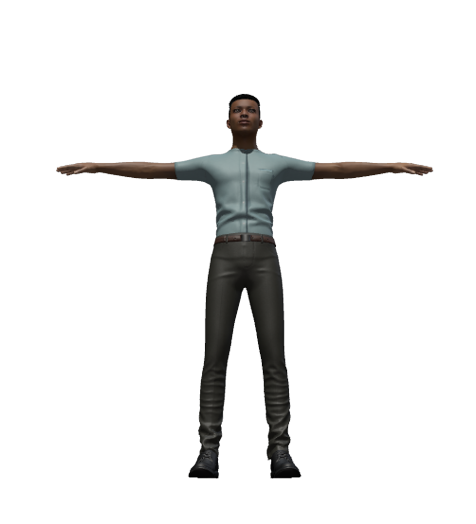
\includegraphics[width=.6\linewidth]{img/assets/remi.png}
  \captionof{figure}{\emph{Personnage masculin}}
  \label{fig:rémi}
\end{minipage}%
\begin{minipage}{.5\textwidth}
  \centering
  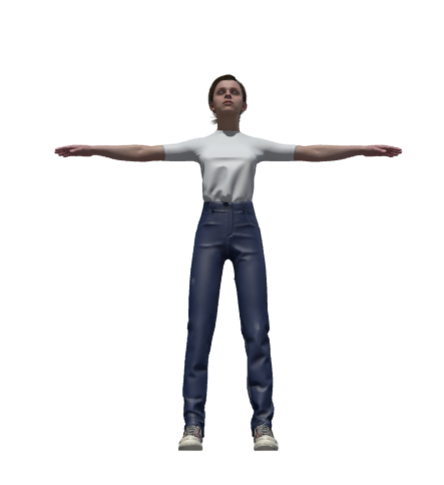
\includegraphics[width=.6\linewidth]{img/assets/sonia.png}
  \captionof{figure}{\emph{Personnage féminin}}
  \label{fig:sonia}
\end{minipage}
\end{figure}

Pour l'entité, un modèle a déjà été choisi. (c.f. I.A. - Intelligence Artificielle)
\vfill
\noindent\makebox[\linewidth]{\rule{.8\paperwidth}{.6pt}}\\[0.2cm]
EPITA Toulouse - Projet S2 - 2022 \hfill Nyctalopia - gameHUB
\noindent\makebox[\linewidth]{\rule{.8\paperwidth}{.6pt}}
\newpage



\subsection{Multijoueur}
\setlength{\parindent}{5ex}
Pour le multijoueur nous avons décidé d'utiliser le SDK Steamworks fourni par Steam Inc. N'étant pas pas nativement compatible avec C\#, nous avons dû utiliser une bibliothèque tierce nommée {\emph{Steamworks.NET}}. Ce SDK permet de créer des lobbys et d'intégrer une liste d'amis, qui facilitera la communication entre les deux joueurs étant donné que Steam est la plateforme de vente de jeux vidéos la plus populaire au monde avec 100+ millions de connexions mensuelles.

Avec tout ces outils en place, il nous a suffi de lire la documentation officielle de Steam, et de mettre en place un script consistant à créer et à joindre des lobbys grâces aux boutons présents au sein de l'interface (c.f. UI/UX).

Un chat vocal est aussi présent pour les joueurs étant dans une même salle de jeu. Pour cela, on a utilisé \emph{SteamVoice}, une bibliothèque fournie par Steam.

\vfill
\noindent\makebox[\linewidth]{\rule{.8\paperwidth}{.6pt}}\\[0.2cm]
EPITA Toulouse - Projet S2 - 2022 \hfill Nyctalopia - gameHUB
\noindent\makebox[\linewidth]{\rule{.8\paperwidth}{.6pt}}
\newpage

\subsection{UI/UX - Interface}
\setlength{\parindent}{5ex}
L'interface utilisateur possède trois parties principales, le menu principal, le menu ``Play'' et le menu ``Paramètres''. Ce dernier permet à l'utilisateur de pouvoir régler la résolution, la taille de la fenêtre (fenêtré, borderless ou plein écran), mais également le son et le choix des touches (AZERTY ou QWERTY).
Le menu ``Play'' possède trois boutons, un placé à gauche, permettant au joueur 1 de créer un lobby et de le rejoindre, et à droite deux boutons permettent au joueur 2 de soit, joindre le lobby avec un \emph{CSteamID} (code de lobby délivré par Steam) ou bien en utilisant sa liste d'ami Steam.
Enfin, le menu principal possède deux grands boutons appelant le joueur à soit débuter une nouvelle campagne ou bien de continuer là où il avait sauvegardé pour la dernière fois (c.f. Sauvegardes)

\begin{figure}[H]
\centering
\begin{minipage}{.5\textwidth}
  \centering
  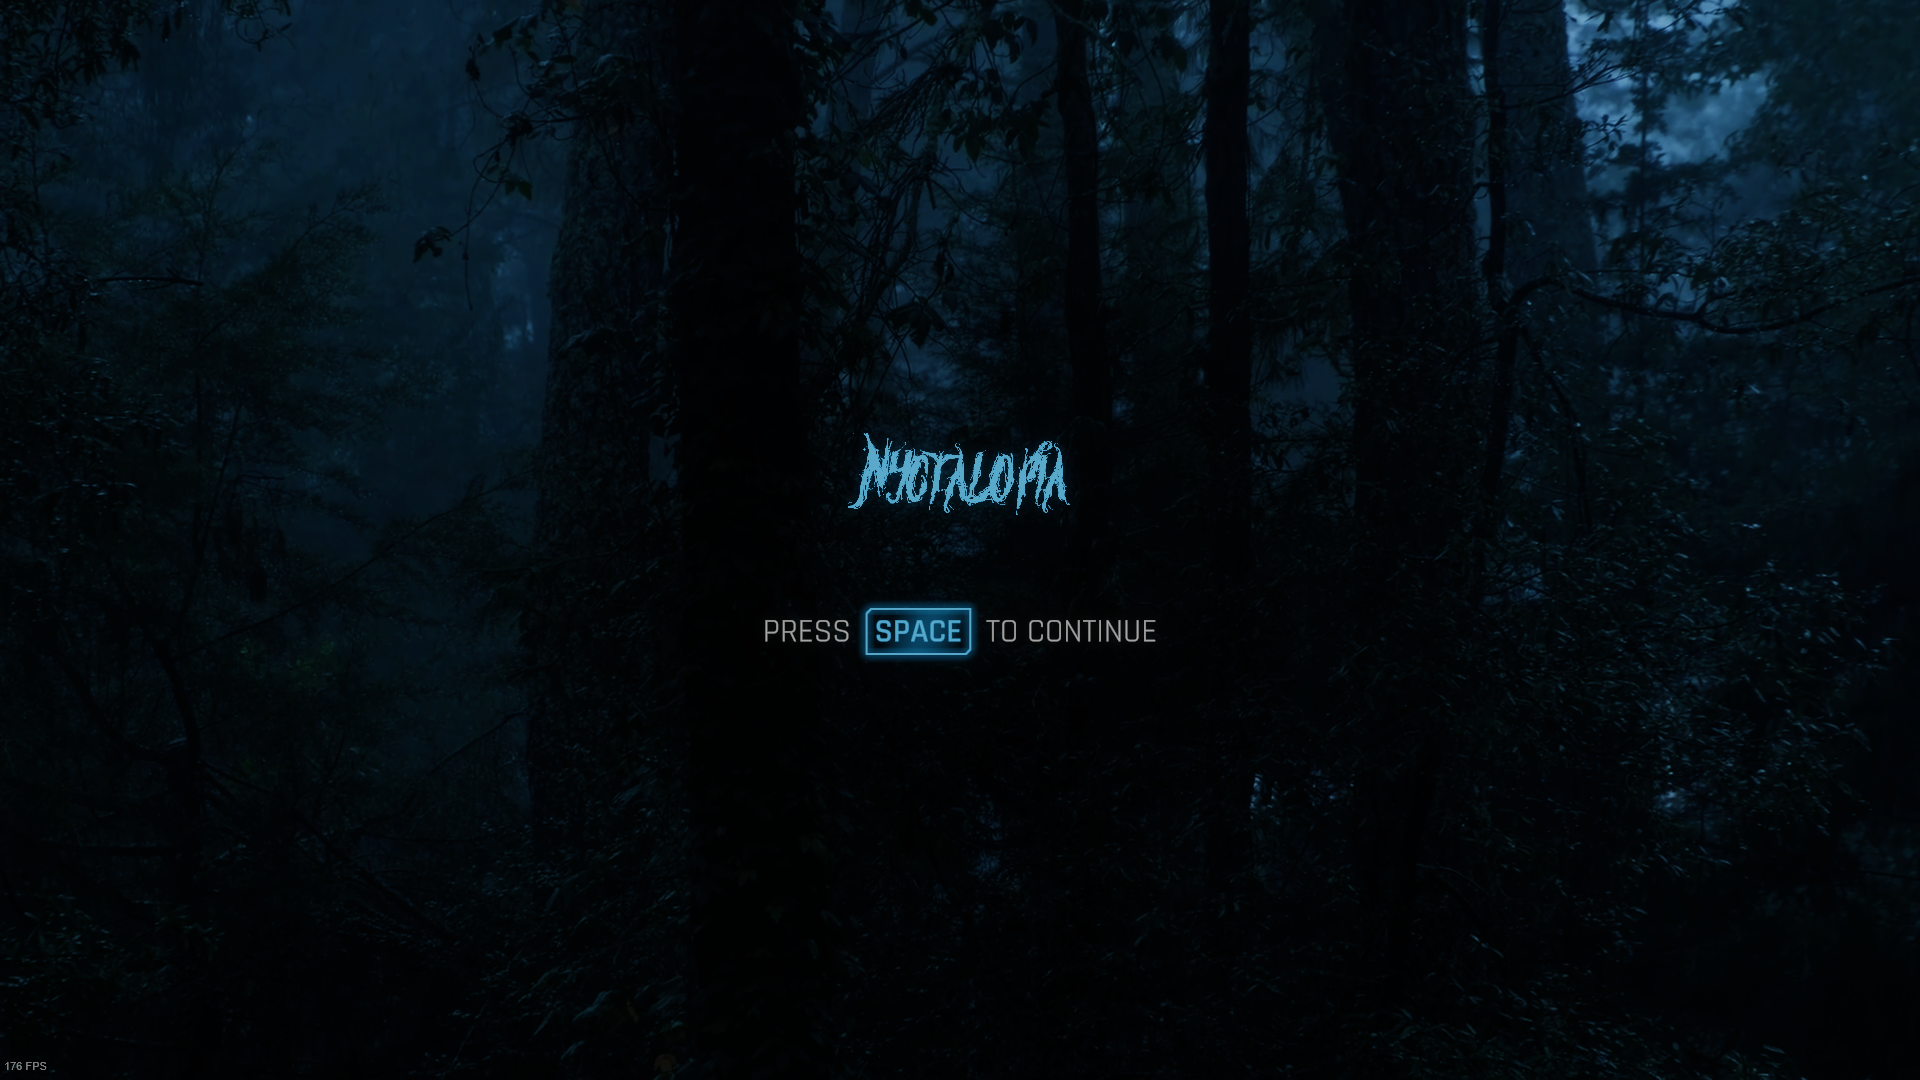
\includegraphics[width=.9\linewidth]{img/ui/UI2.png}
  \captionof{figure}{\emph{Écran d'accueil}}
  \label{fig:uihome}
\end{minipage}%
\begin{minipage}{.5\textwidth}
  \centering
  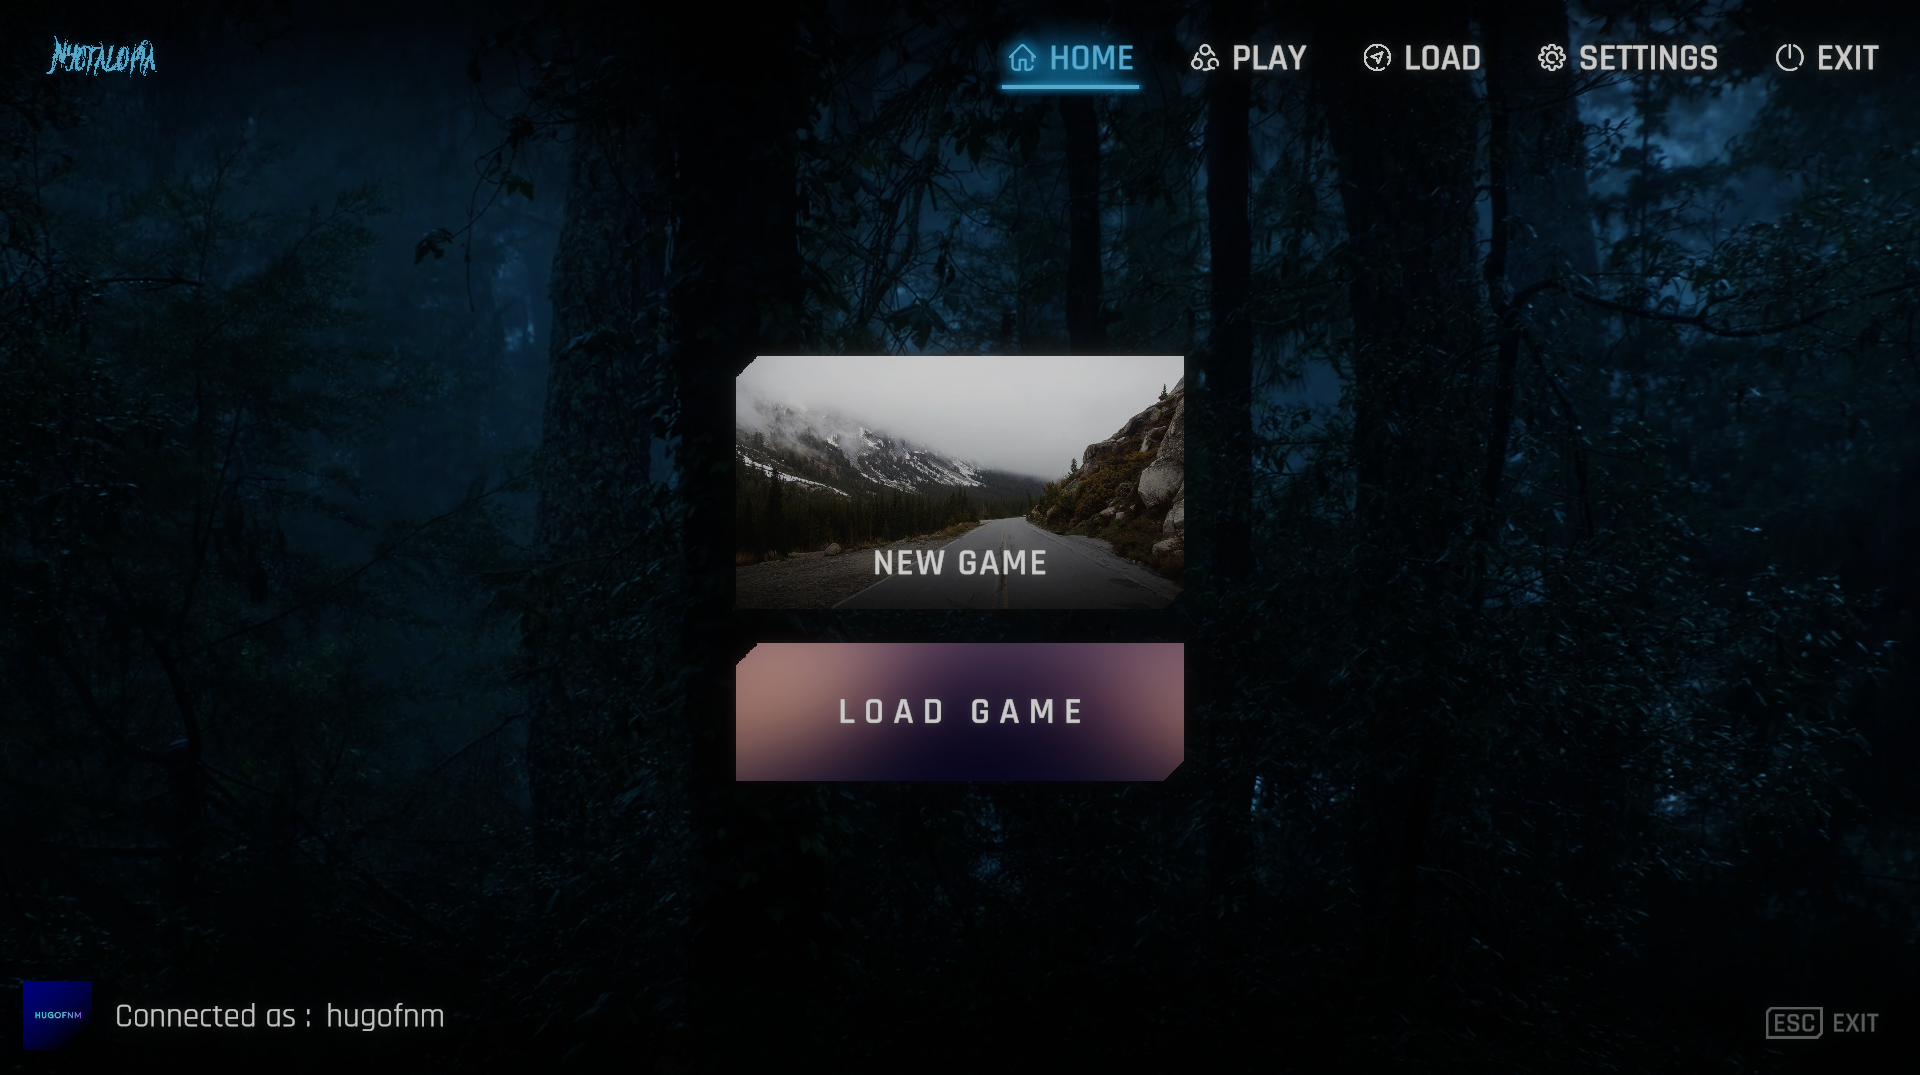
\includegraphics[width=.9\linewidth]{img/ui/UI1.png}
  \captionof{figure}{\emph{Menu principal}}
  \label{fig:uihome2}
\end{minipage}
\end{figure}

\begin{figure}[H]
\centering
\begin{minipage}{.5\textwidth}
  \centering
  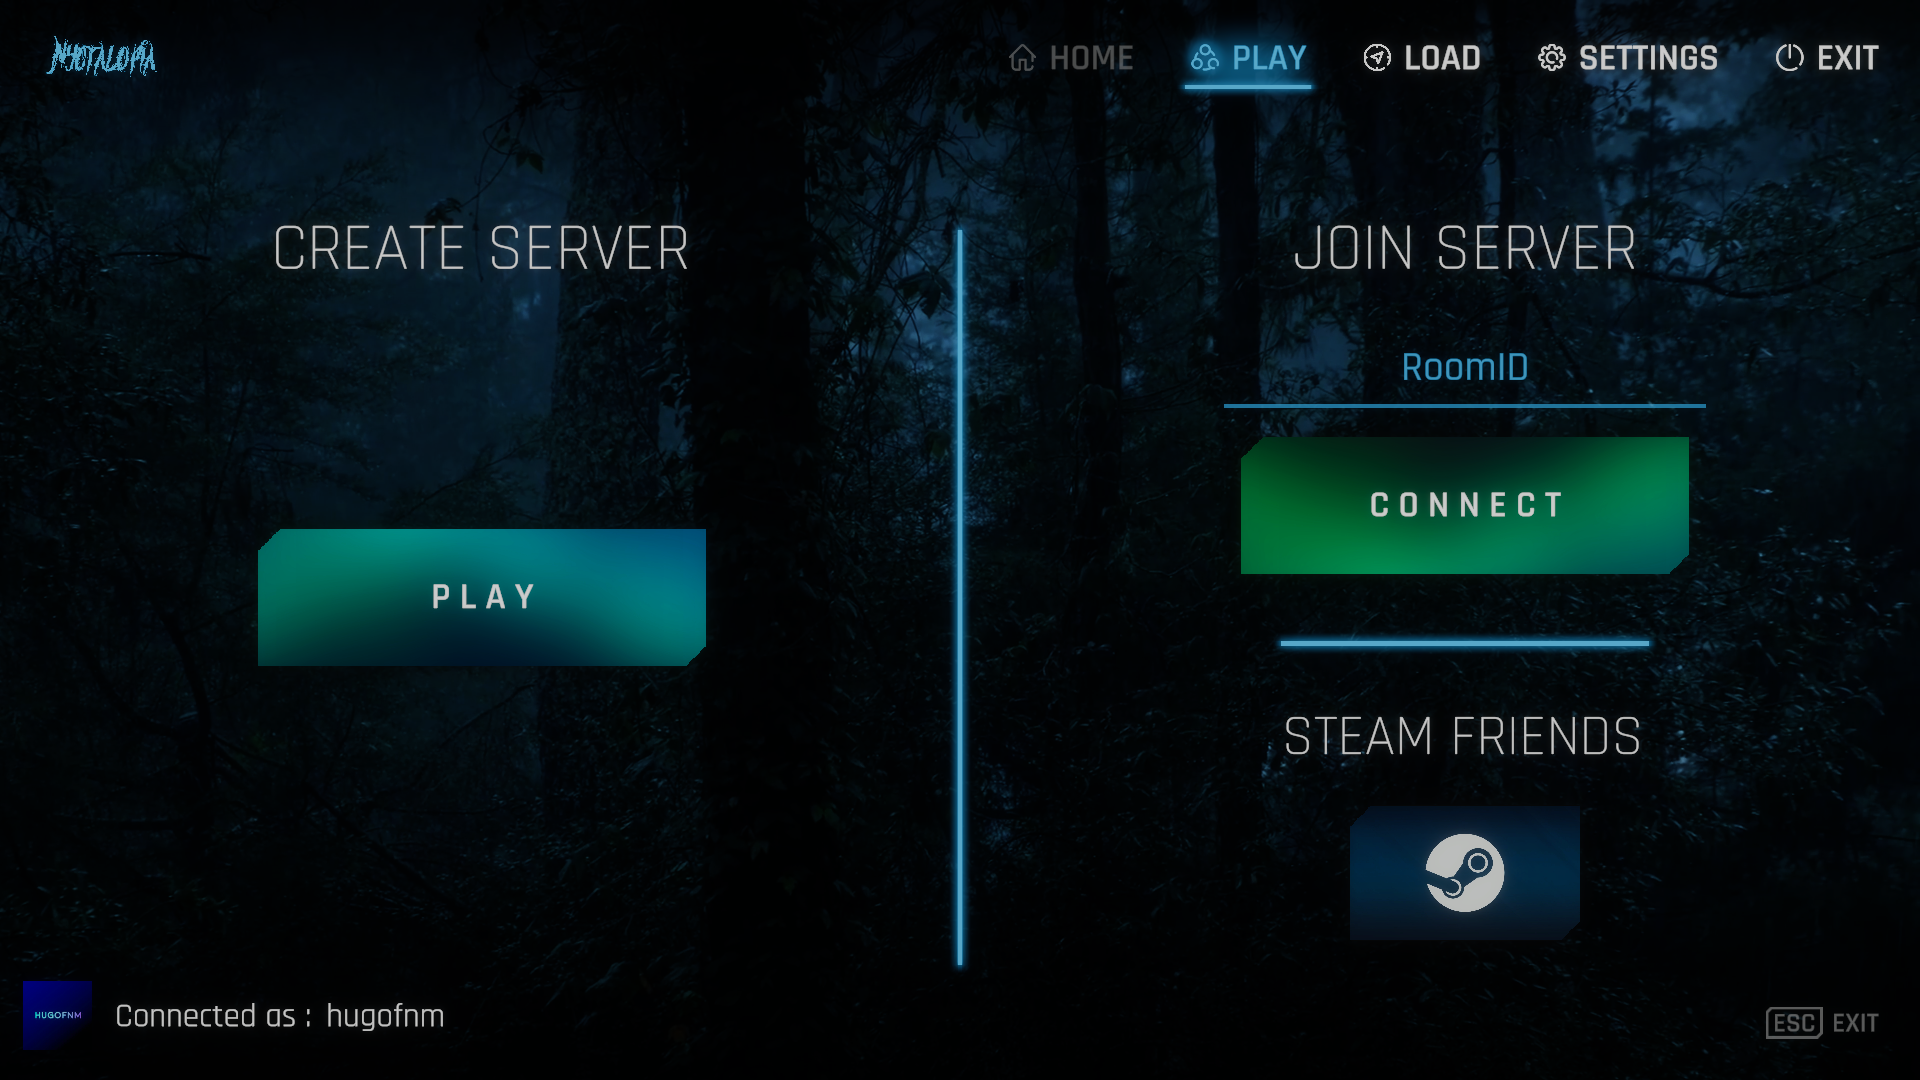
\includegraphics[width=.9\linewidth]{img/ui/UI.png}
  \captionof{figure}{\emph{Menu ``Play''}}
  \label{fig:uiplay}
\end{minipage}%
\begin{minipage}{.5\textwidth}
  \centering
  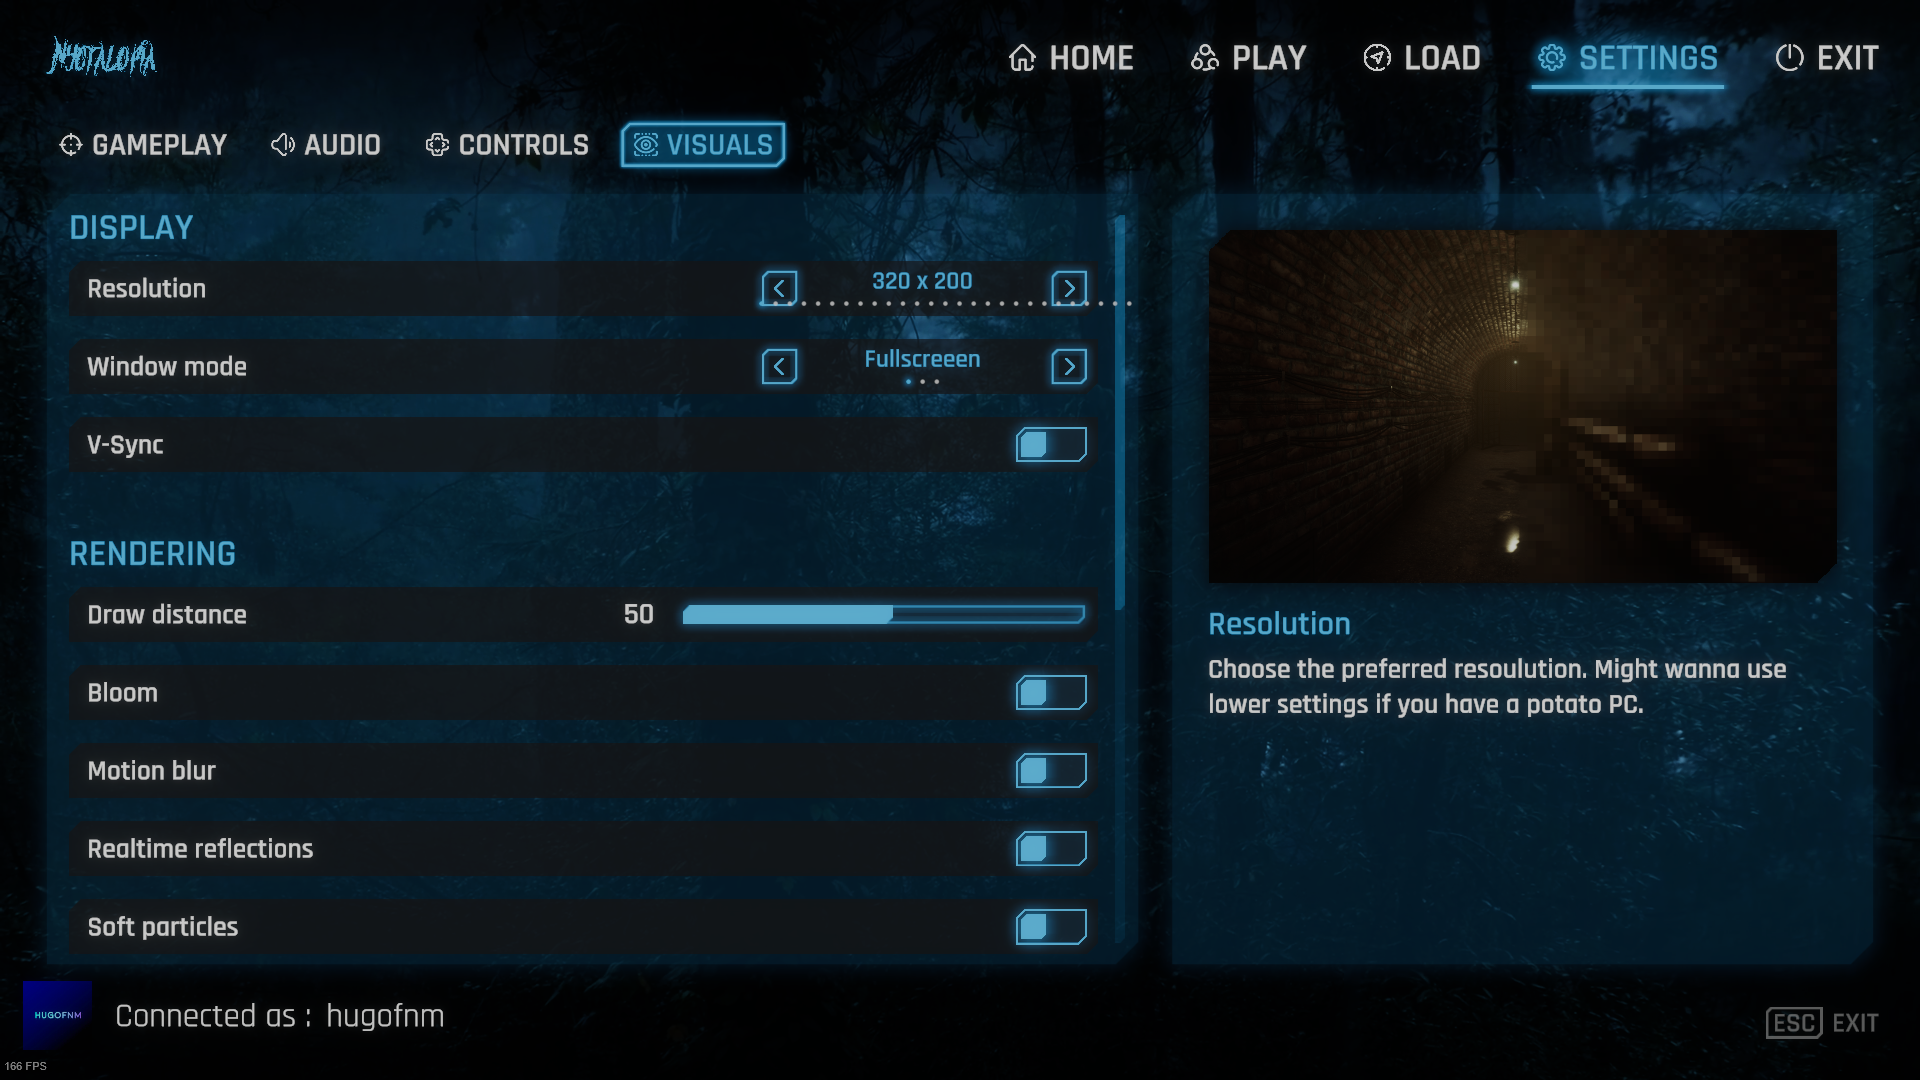
\includegraphics[width=.9\linewidth]{img/ui/UI4.png}
  \captionof{figure}{\emph{Menu ``Paramètres''}}
  \label{fig:uisettings}
\end{minipage}
\end{figure}

Il est désormais possible aussi de changer la langue du jeu. Trois options sont possibles : français, anglais ou espagnol.

\begin{figure}[H]
\centering
\begin{minipage}{.5\textwidth}
  \centering
  \centerline{
\includegraphics[width=2\linewidth]{img/uwufolder/fr.png}}
  \captionof{figure}{\emph{Français}}
  \label{fig:fr}
\end{minipage}%
\end{figure}

\vfill
\noindent\makebox[\linewidth]{\rule{.8\paperwidth}{.6pt}}\\[0.2cm]
EPITA Toulouse - Projet S2 - 2022 \hfill Nyctalopia - gameHUB
\noindent\makebox[\linewidth]{\rule{.8\paperwidth}{.6pt}}

\begin{figure}[H]
\centering
\begin{minipage}{.5\textwidth}
  \centering
  \centerline{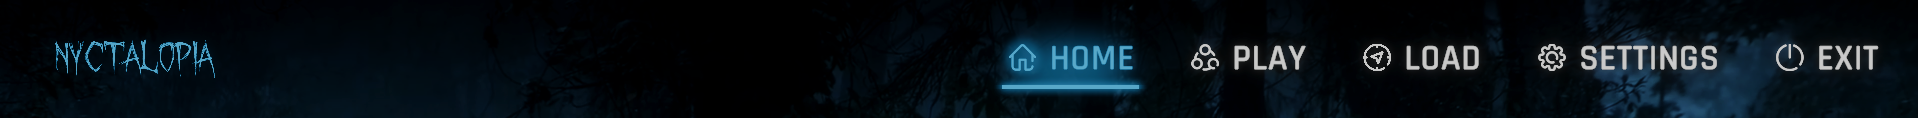
\includegraphics[width=2\linewidth]{img/uwufolder/en.png}}
  \captionof{figure}{\emph{Anglais}}
  \label{fig:en}
\end{minipage}%
\end{figure}

\begin{figure}[H]
\centering
\begin{minipage}{.5\textwidth}
  \centering
  \centerline{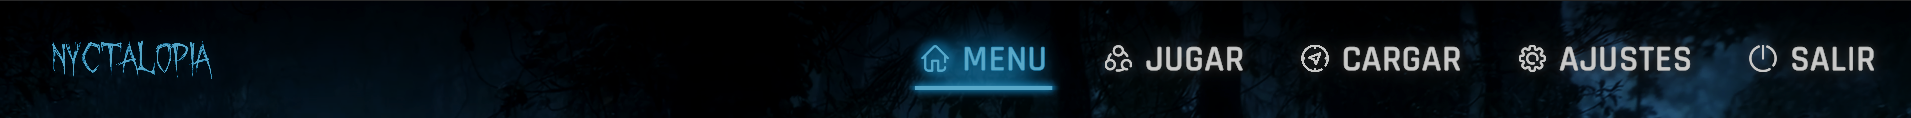
\includegraphics[width=2\linewidth]{img/uwufolder/es.png}}
  \captionof{figure}{\emph{Espagnol}}
  \label{fig:es}
\end{minipage}%
\end{figure}

Si l'utilisateur n'a pas effectué de choix, la langue par défaut sera réglée par rapport à la langue système (le système d'exploitation envoie au jeu la langue principale du système).

\begin{figure}[H]
\centering
\begin{minipage}{.5\textwidth}
  \centering
  \centerline{
\includegraphics[width=1\linewidth]{img/uwufolder/selector.png}}
  \captionof{figure}{\emph{Sélection de la langue dans le menu Paramètres}}
  \label{fig:languageselector}
\end{minipage}%
\end{figure}

Nous avons également mis en place un installateur graphique \emph{``.exe''} qui est accessible à tout utilisateur possédant une machine Windows ou Linux 64 Bits sur le site \emph{get.nyctalopia.games} (c.f Site Web). Ainsi qu'un script permettant d'informer ses amis que l'on joue à Nyctalopia sur la plateforme Discord a été créé.

\begin{figure}[H]
\centering
\begin{minipage}{.5\textwidth}
  \centering
  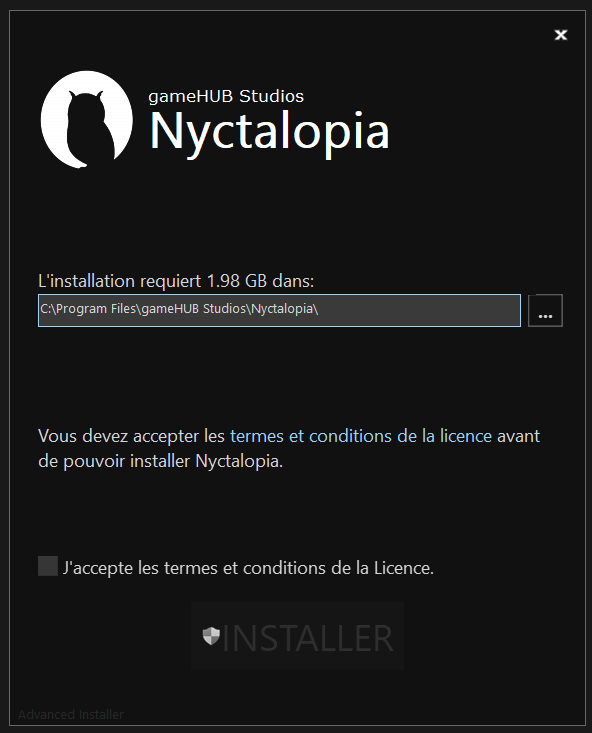
\includegraphics[width=.7\linewidth]{img/ui/installer.png}
  \captionof{figure}{\emph{Installateur Graphique \emph{.exe}}}
  \label{fig:uiinstall}
\end{minipage}%
\begin{minipage}{.5\textwidth}
  \centering
  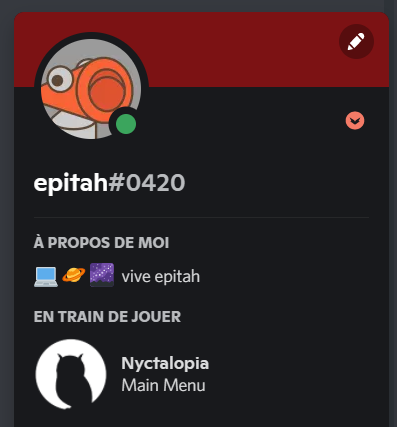
\includegraphics[width=.9\linewidth]{img/ui/DRPC.png}
  \captionof{figure}{\emph{Discord Rich Presence}}
  \label{fig:drpc}
\end{minipage}
\end{figure}

\vfill
\noindent\makebox[\linewidth]{\rule{.8\paperwidth}{.6pt}}\\[0.2cm]
EPITA Toulouse - Projet S2 - 2022 \hfill Nyctalopia - gameHUB
\noindent\makebox[\linewidth]{\rule{.8\paperwidth}{.6pt}}
\newpage

\subsection{Manuels d'instructions et d'installation}
\setlength{\parindent}{5ex}
Nos manuels d'instructions et d'installation sont entièrement complets et vont permettre aux utilisateurs qui rencontreront des problèmes d'avoir tout de suite des réponses à leurs questions. On y retrouve une version en français mais aussi en anglais.
Les utilisateurs pourront retrouver ces manuels sur la page de support du site web.


\begin{figure}[H]
\centering
\begin{minipage}{.5\textwidth}
  \centering
  \centerline{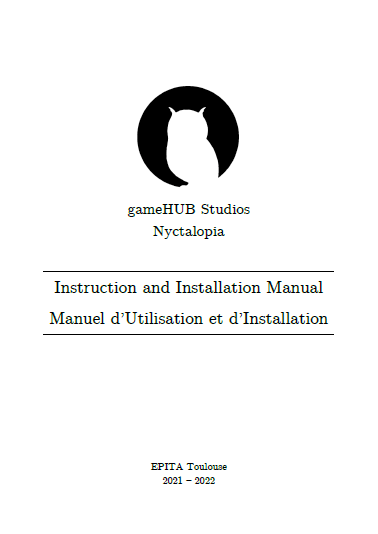
\includegraphics[width=0.8\linewidth]{img/M1.png}}
  \captionof{figure}{\emph{Première page}}
  \label{fig:manual}
\end{minipage}%
\end{figure}


\begin{figure}[H]
\centering
\begin{minipage}{.5\textwidth}
  \centering
  \centerline{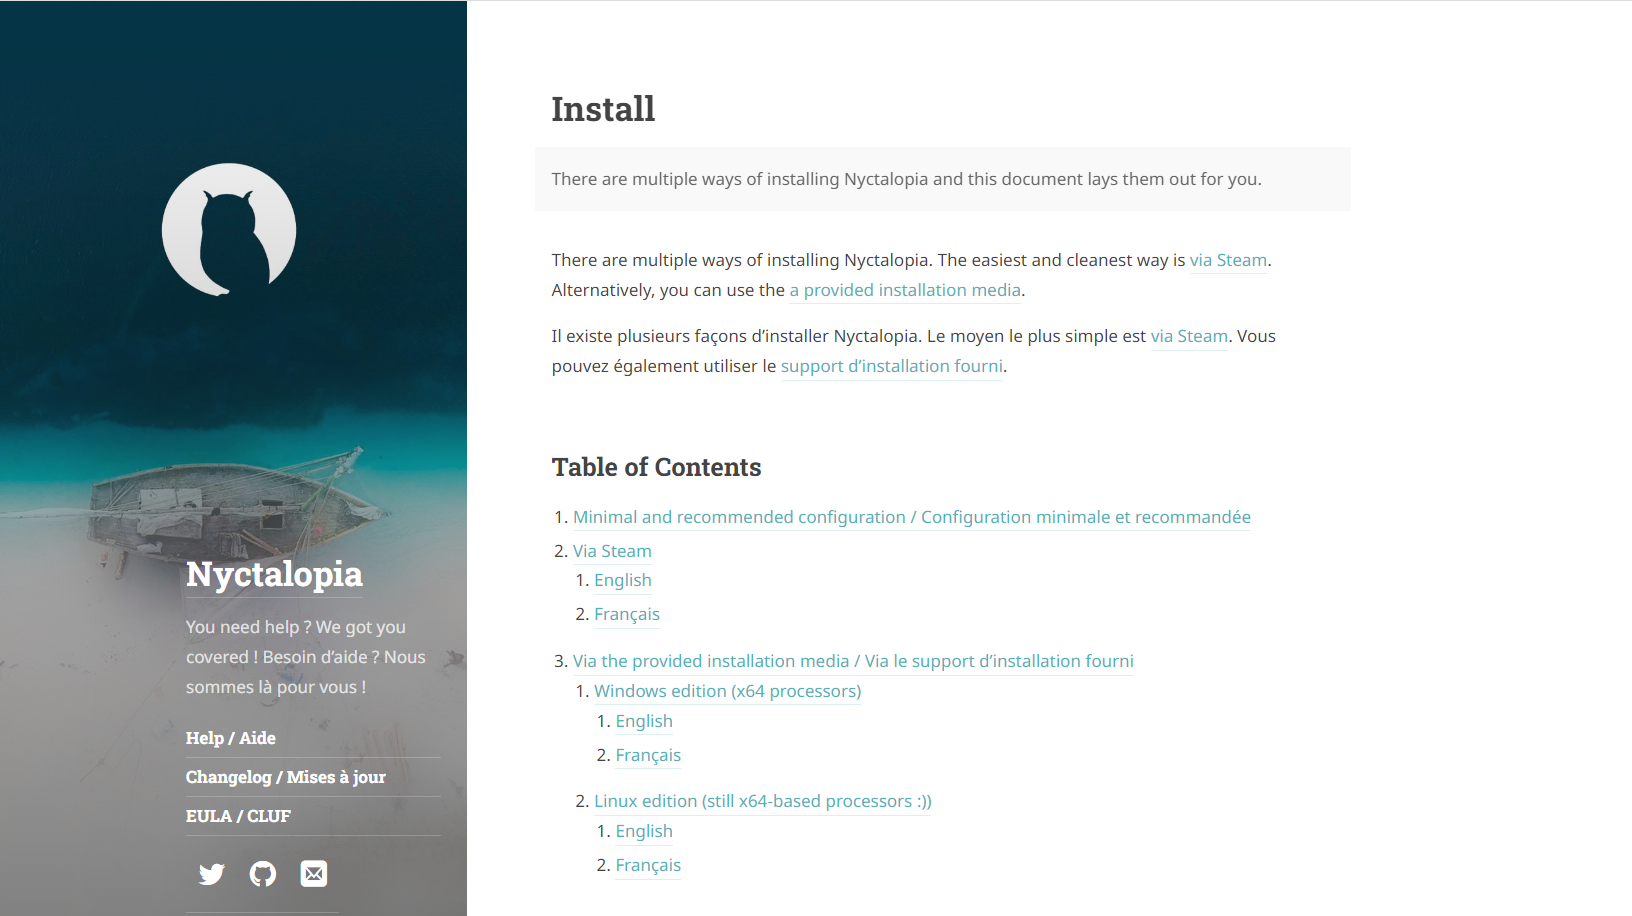
\includegraphics[width=0.8\linewidth]{img/4.PNG}}
  \captionof{figure}{\emph{Manuels d'instructions et d'installation sur le site web}}
  \label{fig:manual}
\end{minipage}%
\end{figure}


\vfill
\noindent\makebox[\linewidth]{\rule{.8\paperwidth}{.6pt}}\\[0.2cm]
EPITA Toulouse - Projet S2 - 2022 \hfill Nyctalopia - gameHUB
\noindent\makebox[\linewidth]{\rule{.8\paperwidth}{.6pt}}
\newpage

\subsection{Site Web}
\setlength{\parindent}{5ex} 
Notre site web est entièrement prêt au public. 
Nous avons également rajouté une page de support pour guider et aider les utilisateurs. Grâce à cette page ils pourront  nous contacter, savoir comment marche le multijoueur, trouver des informations sur l'installation de Nyctalopia et retrouver la licence et condition d'utilisation du jeu. Cette fois le fond du site est agréable visuellement pour permettre aux utilisateurs de facilement lire les différentes informations présente sur cette page.

Nous avons essayé de rendre le site attractif. On peut le voir avec les effets qui permettent que l'arrière-plan et les images au premier plan ne défile pas à la même vitesse ou encore avec le curseur qui suit la souris. Pour ces effets, on a fait le choix d'utiliser des scripts JavaScript pour donner au site un aspect professionnel. De plus, le code HTML est très bien organisé pour nous permettre de l'améliorer ou de le modifier à tout moment. 
Nous avons choisi un thème sombre pour tout de suite mettre le joueur dans l'ambiance du jeu où il sera dans l'obscurité. 
Le site est complètement responsive, donc adapté à tout type d'écran pour permettre au joueurs de le consulter depuis n'importe où. 
A travers ce site, nous cherchons attirer les possibles joueurs en leur donnant envie de jouer à notre jeu, le tout en montrant notre professionnalisme.

\noindent En terme de contenu sur le site on peut retrouver:
\newline
\begin{itemize}

    \item \textbf{Une page d'accueil} : Forêt animée
    \newline
    
\begin{figure}[H]
\centering
\begin{minipage}{.5\textwidth}
  \centering
  \centerline{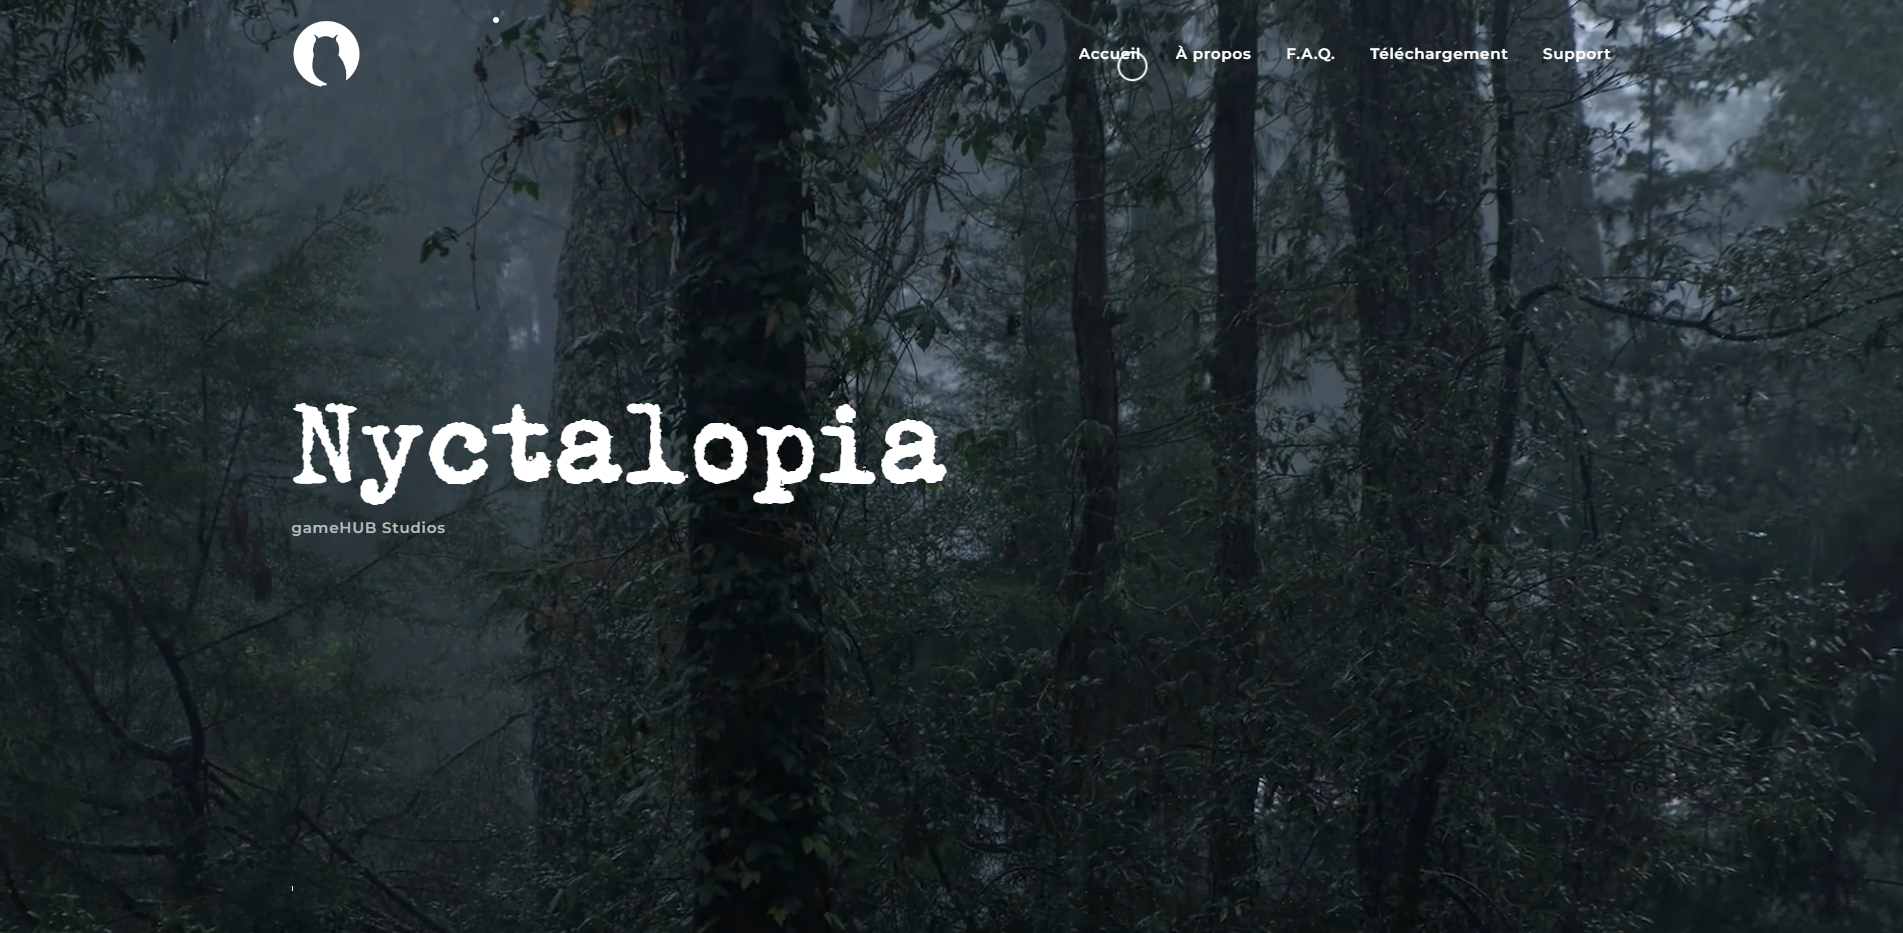
\includegraphics[width=1\linewidth]{img/acceuil.PNG}}
  \captionof{figure}{\emph{Accueil du site}}
  \label{fig:accueil}
\end{minipage}%
\end{figure}


\vfill
\noindent\makebox[\linewidth]{\rule{.8\paperwidth}{.6pt}}\\[0.2cm]
EPITA Toulouse - Projet S2 - 2022 \hfill Nyctalopia - gameHUB
\noindent\makebox[\linewidth]{\rule{.8\paperwidth}{.6pt}}
\newpage


    \item \textbf{Une page de support} : On peut y accéder en appuyant sur \textbf{Support} dans la barre de navigation du site présente sur la page d'accueil.
    \newline
    
\begin{figure}[H]
\centering
\begin{minipage}{.5\textwidth}
  \centering
  \centerline{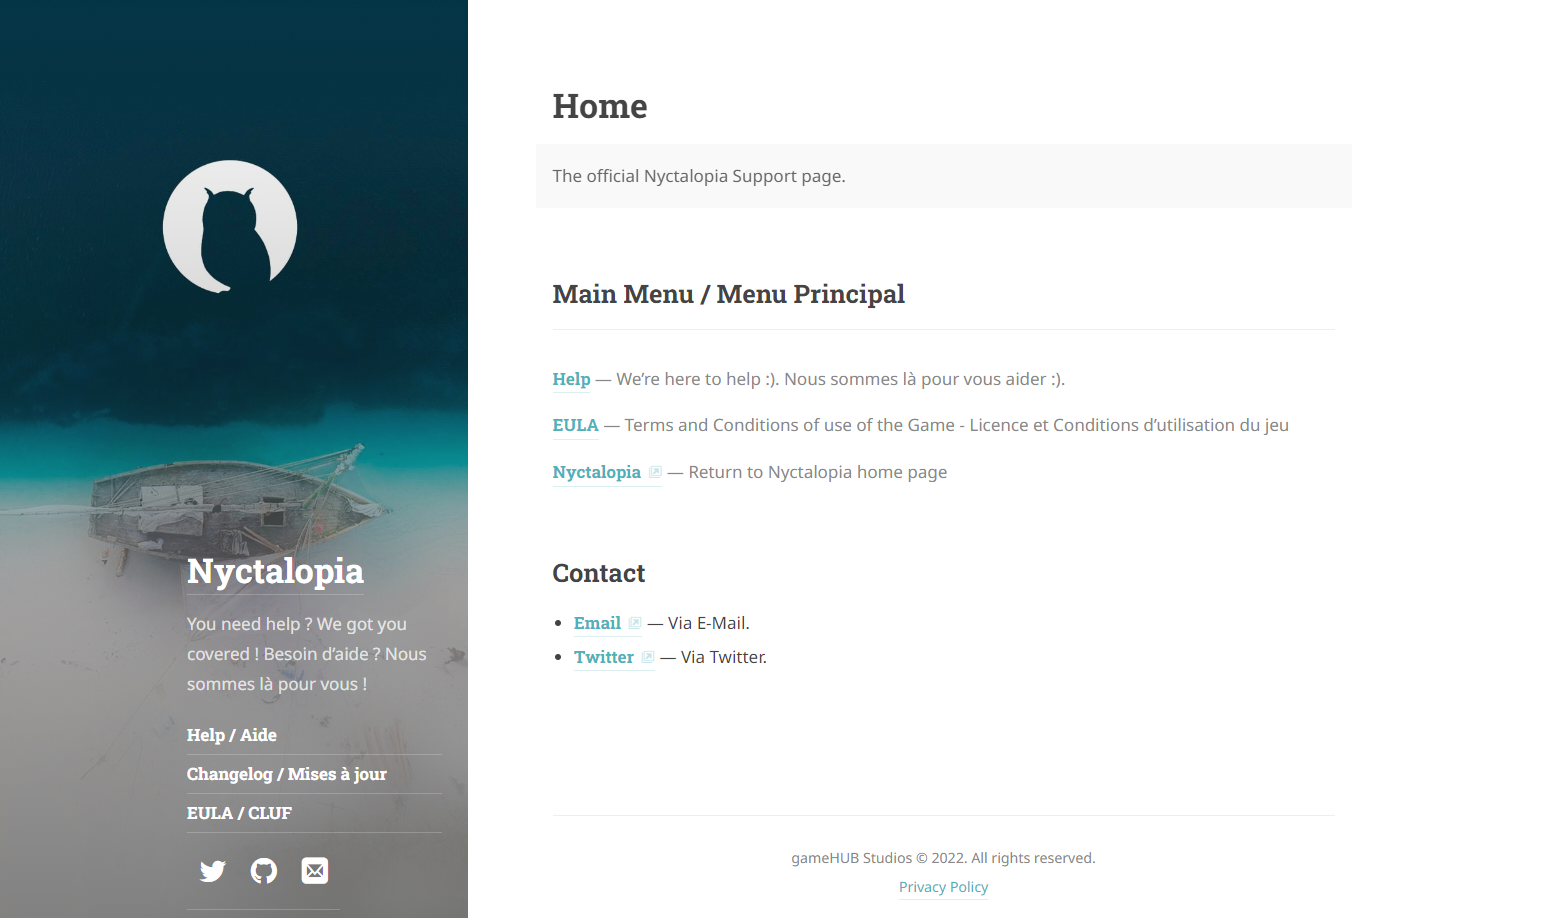
\includegraphics[width=1\linewidth]{img/3.PNG}}
  \captionof{figure}{\emph{Page de support}}
  \label{fig:accueil}
\end{minipage}%
\end{figure}    
    
    \item \textbf{Images du jeu}: Des images de la forêt, l'interface utilisateur ou la scène d'introduction.
    \newline
    
\begin{figure}[H]
\centering
\begin{minipage}{.5\textwidth}
  \centering
  \centerline{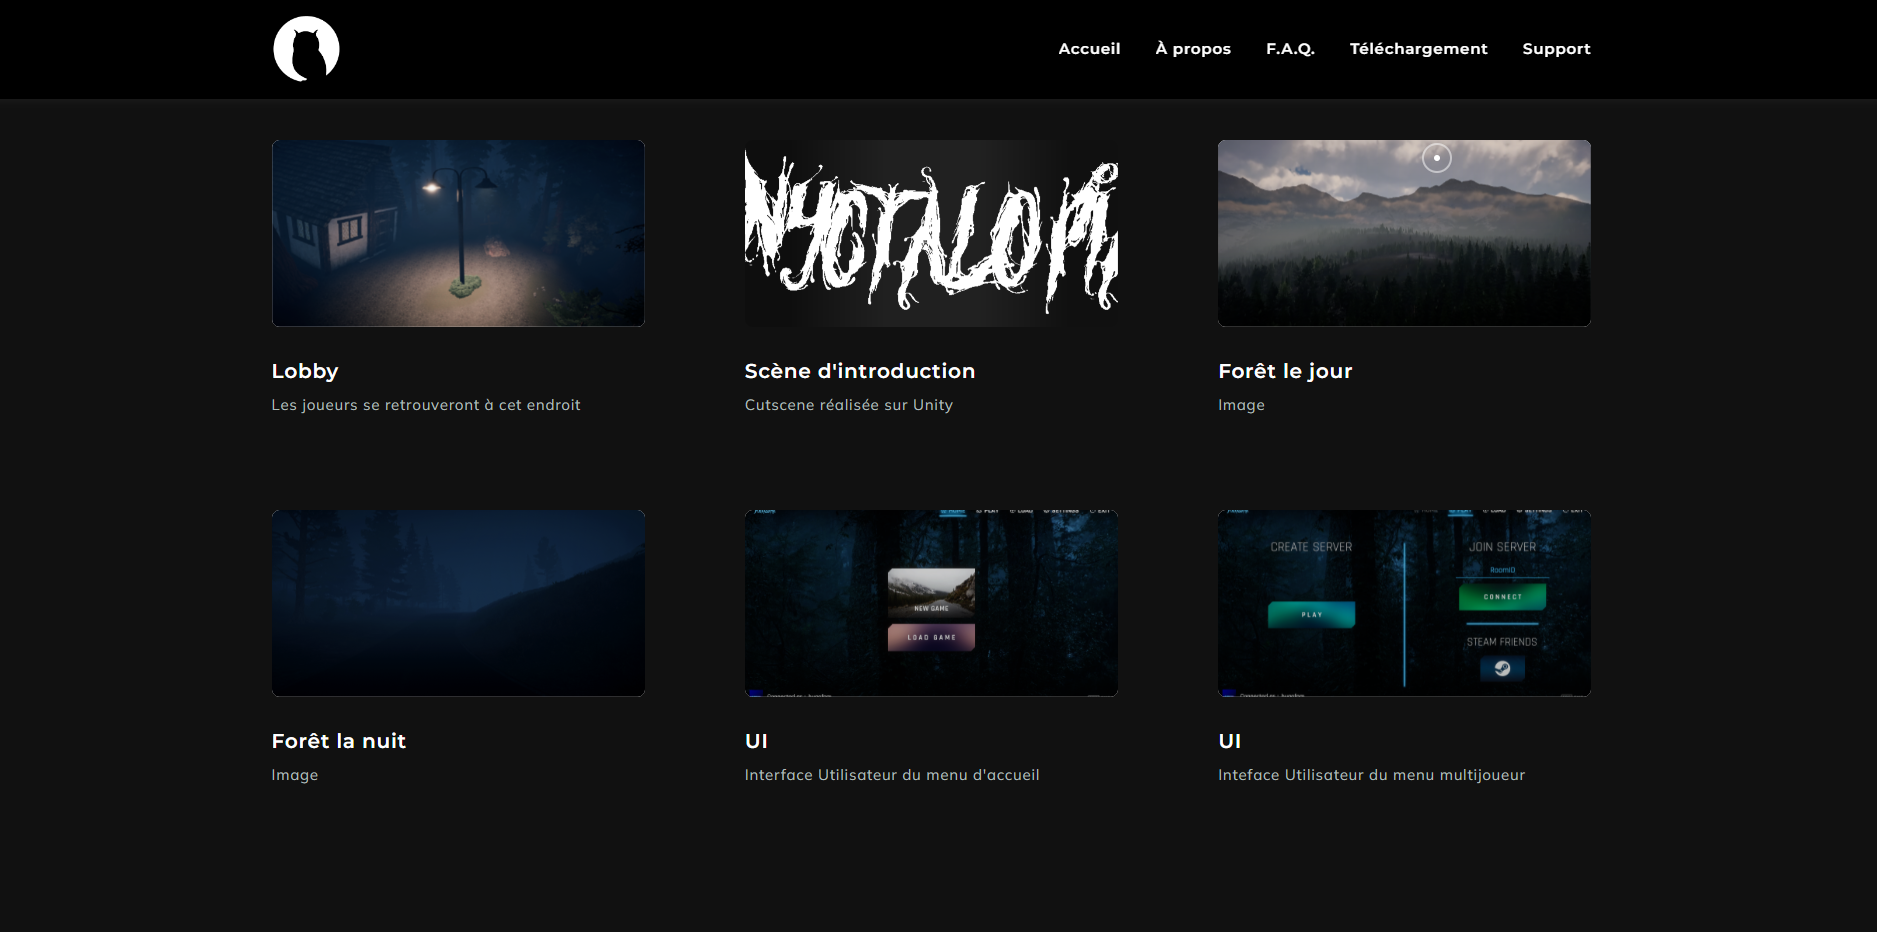
\includegraphics[width=1\linewidth]{img/1.PNG}}
  \captionof{figure}{\emph{Images du jeu}}
  \label{fig:imggame}
\end{minipage}%
\end{figure}

    \item \textbf{Contact} : Un formulaire dans lequel l'utilisateur écrit ses coordonnées et un bouton \textbf{Envoyer} qui renvoie le message écrit dans le cadre de texte vers notre boite mail.
    \newline
    
\begin{figure}[H]
\centering
\begin{minipage}{.5\textwidth}
  \centering
  \centerline{
\includegraphics[width=1\linewidth]{img/Contact.png}}
  \captionof{figure}{\emph{Contact}}
  \label{fig:contact}
\end{minipage}%
\end{figure}


\vfill
\noindent\makebox[\linewidth]{\rule{.8\paperwidth}{.6pt}}\\[0.2cm]
EPITA Toulouse - Projet S2 - 2022 \hfill Nyctalopia - gameHUB
\noindent\makebox[\linewidth]{\rule{.8\paperwidth}{.6pt}}
\newpage

    \item \textbf{Équipe} : Les rôles de chaque membre.
    \newline

\begin{figure}[H]
\centering
\begin{minipage}{.5\textwidth}
  \centering
  \centerline{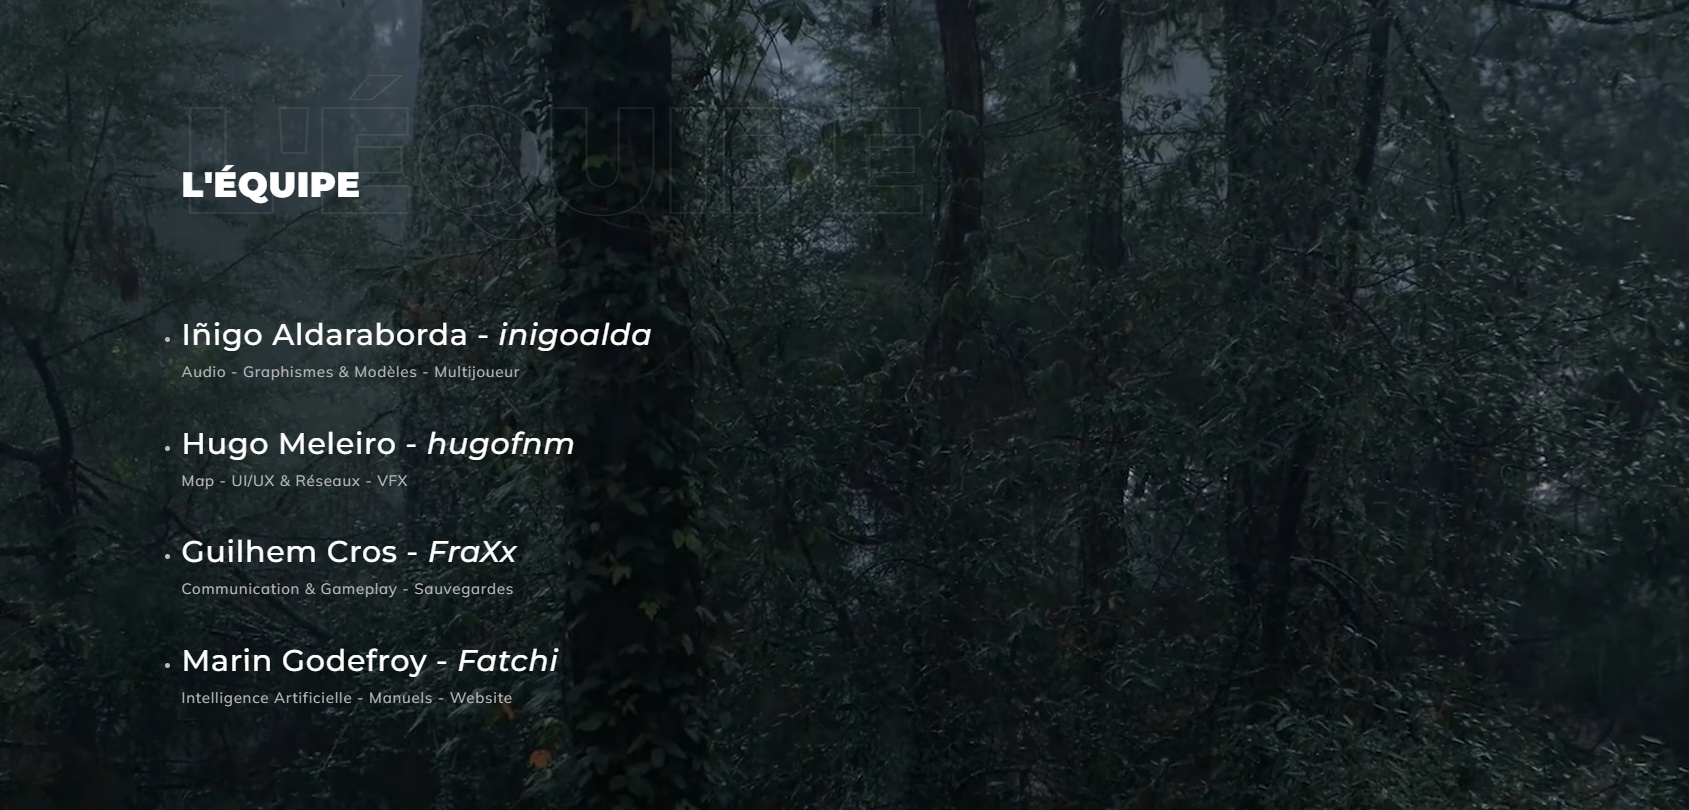
\includegraphics[width=1\linewidth]{img/team.PNG}}
  \captionof{figure}{\emph{Membres du studio GameHub}}
  \label{fig:team}
\end{minipage}%
\end{figure}
    

    \item \textbf{F.A.Q} : Les questions fréquemment posées.
    \newline

\begin{figure}[H]
\centering
\begin{minipage}{.5\textwidth}
  \centering
  \centerline{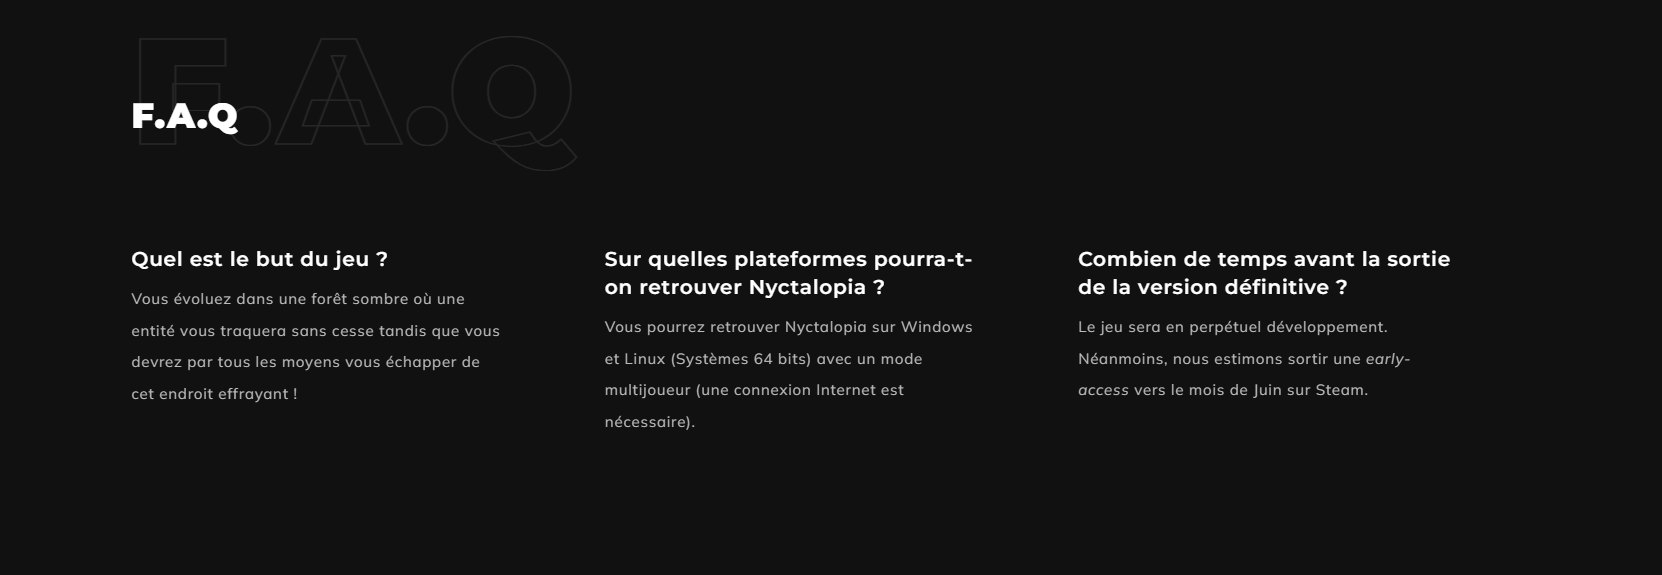
\includegraphics[width=1\linewidth]{img/faq.PNG}}
  \captionof{figure}{\emph{F.A.Q}}
  \label{fig:faq}
\end{minipage}%
\end{figure}

    \item \textbf{Téléchargements} : Lorsque l'utilisateur clique sur le lien \textbf{Télécharger Nyctalopia} il arrive sur cette page qui propose deux méthodes de téléchargement du jeu. Un lien pour le télécharger sur Steam et un lien Windows ou Linux suivant votre système d'exploitation.
    \newline

\begin{figure}[H]
\centering
\begin{minipage}{.5\textwidth}
  \centering
  \centerline{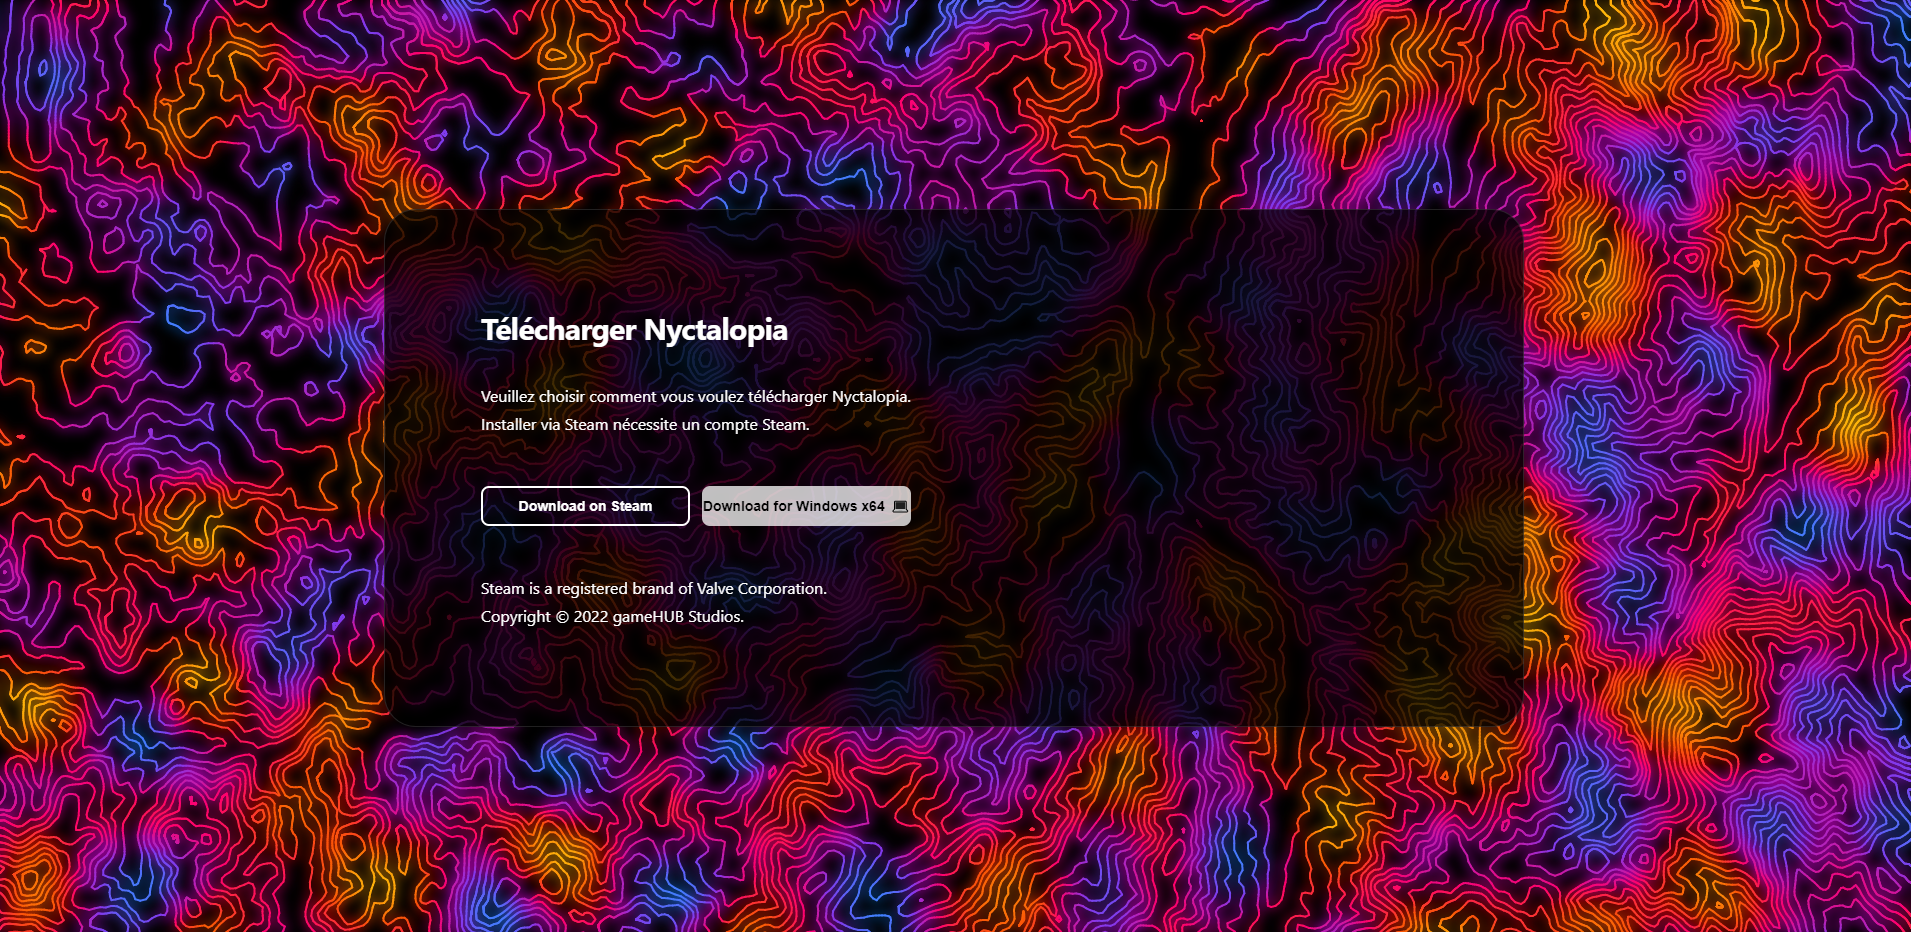
\includegraphics[width=1\linewidth]{img/7.PNG}}
  \captionof{figure}{\emph{Téléchargements}}
  \label{fig:faq}
\end{minipage}%
\end{figure}


\vfill
\noindent\makebox[\linewidth]{\rule{.8\paperwidth}{.6pt}}\\[0.2cm]
EPITA Toulouse - Projet S2 - 2022 \hfill Nyctalopia - gameHUB
\noindent\makebox[\linewidth]{\rule{.8\paperwidth}{.6pt}}
\newpage


    \item \textbf{Annexe} : On y retrouve les liens vers la différente documentation du projet ainsi que des informations diverses.
    
\begin{figure}[H]
\centering
\begin{minipage}{.5\textwidth}
  \centering
  \centerline{
\includegraphics[width=1\linewidth]{img/uwufolder/annexe.png}}
  \captionof{figure}{\emph{Annexe}}
  \label{fig:faq}
\end{minipage}%
\end{figure}
\end{itemize}
\newline

Le site web est hébergé sur CloudFlare Pages, un service gratuit de l'entreprise de gestion DNS CloudFlare, permettant de déployer rapidement à partir d'un repo Git, un site web statique rapide grâce aux serveurs CDN disposés partout dans le monde et sécurisé par un certificat SSL et une protection anti-DDOS.
Le nom de domaine choisi est \emph{nyctalopia.games}. Il est simple et facile à retenir pour l'utilisateur.

\begin{figure}[H]
\centering
\begin{minipage}{.5\textwidth}
  \centering
  \centerline{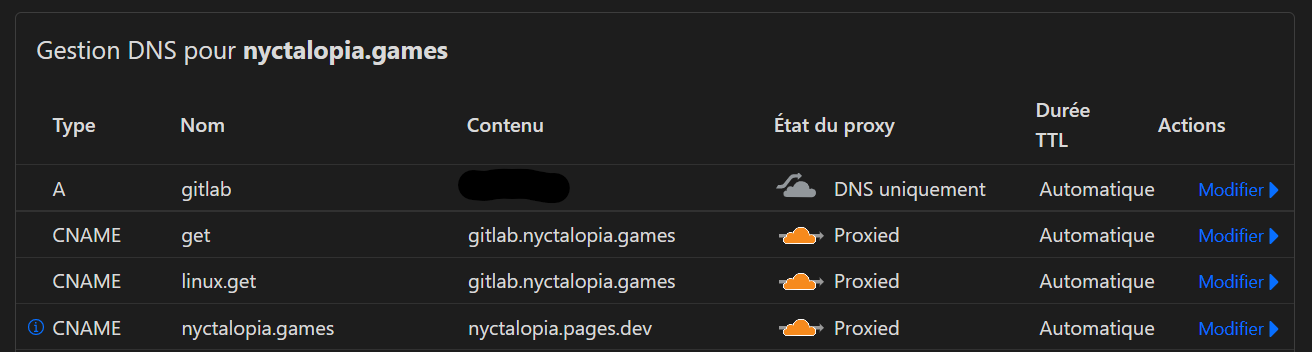
\includegraphics[width=2\linewidth]{img/ui/dns.png}}
  \captionof{figure}{\emph{Interface CloudFlare}}
  \label{fig:dns}
\end{minipage}%
\end{figure}

\begin{figure}[H]
\centering
\begin{minipage}{.5\textwidth}
  \centering
  \centerline{
\includegraphics[width=1.5\linewidth]{img/ssl.png}}
  \captionof{figure}{\emph{Site sécurisé SSL}}
  \label{fig:ssl}
\end{minipage}%
\end{figure}

Nous avons également décidé de mettre en place un GitLab (\emph{gitlab.nyctalopia.games}) privé sur un serveur nous appartenant, ce qui nous a permis d'utiliser la puissance brute de Git LFS et des pipelines CI/CD, améliorant notre productivité sans perdre de temps.

\vfill
\noindent\makebox[\linewidth]{\rule{.8\paperwidth}{.6pt}}\\[0.2cm]
EPITA Toulouse - Projet S2 - 2022 \hfill Nyctalopia - gameHUB
\noindent\makebox[\linewidth]{\rule{.8\paperwidth}{.6pt}}

\newpage